\documentclass[headrule,footrule]{foils}

%%
%%%  Macros
%%%
\newcommand{\logo}{HG2002 (2020)}
\usepackage[hidelinks]{hyperref}

\newcommand{\header}[3]{%
  \title{\vspace*{-2ex} \large 
    HG2002 Semantics and Pragmatics
% \thanks{Creative
%       Commons Attribution License: 
%       you are free to share and adapt as long as you give 
%       appropriate credit and add no additional restrictions: 
%       \protect\url{https://creativecommons.org/licenses/by/4.0/}.
%     }
    \\[2ex] \Large  \emp{#2} \\ \emp{#3}}
  \author{\blu{Francis Bond}   \\ 
    \normalsize  \textbf{Division of Linguistics and Multilingual Studies}\\
    \normalsize  \url{http://www3.ntu.edu.sg/home/fcbond/}\\
    \normalsize  \texttt{bond@ieee.org}}
  \MyLogo{\logo}
  % \MyLogo{奈良女子大学:欧米言語情報理論II}
  \date{#1
    \\  \url{https://bond-lab.github.io/Semantics-and-Pragmatics/}
\\[.5ex] \footnotesize Creative  Commons Attribution License:  you are free to share and adapt 
\\[-.25ex] \footnotesize   as long as you give    appropriate credit and add no
additional restrictions: 
\\ \small  \protect\url{https://creativecommons.org/licenses/by/4.0/}.
}
  % \renewcommand{\logo}{#2}
  % \special{! /pdfmark where
  %   {pop} {userdict /pdfmark /cleartomark load put} ifelse
  %   [ /Author (Francis Bond)
  %   /Title (#1: #2)
  %   /Subject (HG2002: Semantics and Pragmatics)
  %   /Keywords (Semantics, Pragmatics, Meaning)
  %   /DOCINFO pdfmark}
  %   }
  \hypersetup{%
    final       = true,
    colorlinks  = true,
    urlcolor    = blue,
    citecolor   = blue,
    linkcolor   = MidnightBlue,
    unicode     = true,
    pdfauthor   = {Francis Bond},
    pdfkeywords = {Semantics, Pragmatics, Meaning},
    pdftitle    = {#1: #2},
    pdfsubject  = {HG2002 Semantics and Pragmatics; License CC BY 4.0}
  }
}


\usepackage[a4paper,landscape]{geometry}
%\usepackage[dvips]{xcolor}
\usepackage[dvipsnames,x11names]{xcolor}
\usepackage{graphicx}
\newcommand{\blu}[1]{\textcolor{blue}{#1}}
\newcommand{\grn}[1]{\textcolor{green}{#1}}
\newcommand{\hide}[1]{\textcolor{white}{#1}}
\newcommand{\emp}[1]{\textcolor{red}{#1}}
\newcommand{\txx}[1]{\textbf{\textcolor{blue}{#1}}}
\newcommand{\lex}[1]{\textbf{\mtcitestyle{#1}}}


\usepackage{amsmath,latexsym}
\usepackage{pifont}
\renewcommand{\labelitemi}{\textcolor{violet}{\ding{227}}}
\renewcommand{\labelitemii}{\textcolor{purple}{\ding{226}}}

\newcommand{\subhead}[1]{\noindent\textbf{#1}\\[5mm]}

\newcommand{\Bad}{\emp{\raisebox{0.15ex}{\ensuremath{\mathbf{\otimes}}}}}
\newcommand{\bad}{*}

\newcommand{\com}[1]{\hfill \textnormal{(\emp{#1})}}%
\newcommand{\cxm}[1]{\hfill \textnormal{(\txx{#1})}}%
\newcommand{\cmm}[1]{\hfill \textnormal{(#1)}}%

\usepackage{relsize,xspace}
\newcommand{\into}{\ensuremath{\rightarrow}\xspace}
\newcommand{\ent}{\ensuremath{\Rightarrow}\xspace}
\newcommand{\nent}{\ensuremath{\not\Rightarrow}\xspace}
\newcommand{\tot}{\ensuremath{\leftrightarrow}\xspace}
\usepackage{url}
\newcommand{\lurl}[1]{\MyLogo{\url{#1}}}

\usepackage{mygb4e}
\let\eachwordone=\itshape
\newcommand{\lx}[1]{\textbf{\textit{#1}}}
\newcommand{\ix}{\ex\it}

\newcommand{\cen}[2]{\multicolumn{#1}{c}{#2}}
%\usepackage{times}
%\usepackage{nttfoilhead}
\newcommand{\myslide}[1]{\foilhead[-25mm]{\raisebox{12mm}[0mm]{\emp{#1}}}\MyLogo{\logo}}
\newcommand{\myslider}[1]{\rotatefoilhead[-25mm]{\raisebox{12mm}[0mm]{\emp{#1}}}}
%\newcommand{\myslider}[1]{\rotatefoilhead{\raisebox{-8mm}{\emp{#1}}}}

\newcommand{\section}[1]{\myslide{}{\begin{center}\Huge \emp{#1}\end{center}}}



\usepackage[lyons,j,e,k]{mtg2e}
\renewcommand{\mtcitestyle}[1]{\textcolor{teal}{\textsl{#1}}}
%\renewcommand{\mtcitestyle}[1]{\textsl{#1}}
\newcommand{\ja}[1]{\mtcitestyle{\makexeCJKactive #1\makexeCJKinactive}}
\newcommand{\chn}{\mtciteform}
\newcommand{\zsm}{\mtciteform}
%\newcommand{\cmn}[1]{make\cjkactive\mtciteform#1\makecjkinactive}
\newcommand{\iz}[1]{\textup{\texttt{\textcolor{blue}{\textbf{#1}}}}}
\newcommand{\con}[1]{\textsc{#1}}
\newcommand{\gm}{\textsc}
\newcommand{\cmp}[1]{{[\textsc{#1}]}}
\newcommand{\sr}[1]{\ensuremath{\langle}#1\ensuremath{\rangle}}
\usepackage[normalem]{ulem}
\newcommand{\ul}{\uline}
\newcommand{\ull}{\uuline}
\newcommand{\wl}{\uwave}
\newcommand{\vs}{\ensuremath{\Leftrightarrow}~}
%%% theta role
\newcommand{\tr}[1]{\textcolor{Chartreuse4}{\textsc{#1}}}
%%% theta grid
\newcommand{\grid}[1]{\ensuremath{\langle}\tr{#1}{\ensuremath{\rangle}}}

%%%
%%% Bibliography
%%%
\usepackage{natbib}
%\usepackage{url}
\usepackage{bibentry}
%\usepackage{CJKutf8}


\usepackage{fontenc}
\usepackage{polyglossia}
\setmainlanguage{english}
\setotherlanguages{tamil}
\setmainfont[Ligatures=TeX]{TeX Gyre Pagella}
\setsansfont[Ligatures=TeX]{TeX Gyre Heros}

\usepackage{xeCJK}
\makexeCJKinactive
\newcommand{\zh}[1]{\mtcitestyle{\makexeCJKactive #1\makexeCJKinactive}}
%\newcommand{\ja}[1]{\makexeCJKactive #1\makexeCJKinactive}
\setCJKmainfont{Noto Sans CJK JP}
\setCJKsansfont{Noto Sans CJK SC}
\setCJKmonofont{Noto Sans CJK SC}

\newfontfamily\tamilfont[Script=Tamil]{Noto Sans Tamil}
\newfontfamily\tamilfontsf[Script=Tamil]{Noto Sans Tamil}
\newcommand{\tam}[1]{\texttamil{#1}}
%%% From Tim
\newcommand{\WMngram}[1][]{$n$-gram#1\xspace}
\newcommand{\infers}{$\rightarrow$\xspace}


\usepackage{rtrees,qtree}
\renewcommand{\lf}[1]{\br{#1}{}}
\usepackage{avm}
%\avmoptions{topleft,center}
\newcommand{\ft}[1]{\textsc{#1}}
\newcommand{\val}[1]{\textit{#1}}
\newcommand{\typ}[1]{\textit{#1}}
\avmfont{\sc}
\avmvalfont{\sc}
\renewcommand{\avmtreefont}{\sc}
\avmsortfont{\it}


%%% From CSLI book
\newcommand{\mc}{\multicolumn}
\newcommand{\HD}{\textbf{H}\xspace}
\newcommand{\el}{\< \>}
\makeatother
\long\def\smalltree#1{\leavevmode{\def\\{\cr\noalign{\vskip12pt}}%
\def\mc##1##2{\multispan{##1}{\hfil##2\hfil}}%
\tabskip=1em%
\hbox{\vtop{\halign{&\hfil##\hfil\cr
#1\crcr}}}}}
\makeatletter

%\usepackage{tipa}
\usepackage{multicol}


\newcommand{\task}{\marginpar{\large ~~~\textbf{?}}}
\newcommand{\sh}[1]{\href{https://www.arthur-conan-doyle.com/index.php?title=#1}{#1}}

\usepackage{tikz}
\usepackage{tikz-qtree}

\header{Lecture 12}{Semantics and Pragmatics}{Review}


\usepackage{avm}
\avmoptions{topleft,center}

% \usepackage[lyons,j,e,k]{mtg2e}
% \renewcommand{\mtcitestyle}[1]{\textsl{#1}}
% \newcommand{\iz}[1]{\texttt{\textup{#1}}}
% \newcommand{\gm}{\textsc}
% \newcommand{\ul}{\underline}
% \usepackage[normalem]{ulem}

\usepackage{bibentry}
\usepackage{natbib}
\renewcommand{\cite}{\bibentry}
\begin{document}
\maketitle
\bibliographystyle{plainnat}
\nobibliography{abb,mtg,ling}

%\myslide{Course Overview}
%\input{schedule}
% \begin{center}
% Final in class exam on Nov 20th 10:00--12:00 (2 hours exam) SPMS LT3  
% \end{center}


\myslide{Review Overview}

\begin{itemize}
\item Overall Review
\item Review of the lectures
\item Parting Words
  \begin{center}
    Final in class quiz \\
    Same time and place, next week
  \end{center}
\end{itemize}


\section{Big Picture}

\begin{itemize}
\item Language can be used to convey information
  \begin{itemize}
  \item we model this as \txx{meaning}
  \item \txx{lexical semantics} looks at relations between words in
    the lexicon
  \item \txx{structural semantics} looks at relations between words in
    utterances
  \item \txx{pragmatics} looks at how and why we use words
  \end{itemize}
\item Meaning is infinite
  \begin{itemize}
  \item it can be built up \txx{compositionally}
  \item it can vary and be extended continuously
  \item we can only model it approximately
  \end{itemize}
\end{itemize}


\section{Revision: \\ Introduction to Semantics}

\myslide{What is Semantics}
\begin{itemize}
\item Very broadly, semantics is the study of meaning
  \begin{itemize}
  \item Word meaning
  \item Sentence meaning
  \end{itemize}
\item Layers of Linguistic Analysis
  \begin{enumerate}%\addtolength{\itemsep}{-0.75ex}
  \item Phonetics \& Phonology
  \item Morphology
  \item Syntax
  \item Semantics
  \item Pragmatics
  \end{enumerate}
\item Semantics could be \txx{autonomous} or \txx{integrated} with other knowledge
\end{itemize}

\myslide{Meaning in the larger context}

\begin{itemize}
\item Semiotics is the study of interpreting symbols, or \txx{signification}
  \begin{itemize}
  \item We refer to the \txx{signified}
  \item Using a \txx{signifier}\hfill Saussure
  \end{itemize}
\item Problems with defining meaning
  \begin{itemize}
  \item The \txx{grounding} problem and \txx{circularity}
  \item The boundaries of meaning: \txx{linguistic} vs \txx{encyclopedic knowledge}
  \item Individual variation in meaning: \txx{idiolects}
  \item Words can be combined to form an infinite number of expressions
    \begin{itemize}
    \item This building up of meaning is referred to as \txx{composition}
    \item If the meaning of the whole can be deduced from the parts then it is \txx{compositional}
  \end{itemize}
\end{itemize}
\end{itemize}

\myslide{Metalanguages and Notational Conventions}

We use language to talk about language, which can get messy.  So we
use certain words with very specific technical senses, and we use
fonts to convey information.

\begin{itemize}
\item \eng[gloss]{word} or \eng{utterance} 
  \hfill (\textbf{\emp{do}} this in your assignments!)
\item \lex{lexeme}
\item \iz{predicate}
\item \con{concept}
\item \txx{technical term} $\leftarrow$ remember me!
\end{itemize}

\myslide{Utterances, Sentences and Propositions}

\begin{itemize}
\item \txx{utterance}: an actual instance of saying (or writing  or \ldots) something
\item \txx{sentence}: an abstraction, the type of what was said
  \begin{exe}
    \ex Caesar invades Gaul
  \end{exe}
\item \txx{proposition}: a further abstraction, normally ignoring some non-literal meaning
  \begin{exe}
    \ex \iz{invade(Caesar, Gaul)}
  \end{exe}
  \begin{itemize}
  \item \txx{information structure}: what part of a proposition is emphasized
 \begin{exe}
   \ex Caesar invaded Gaul
   \ex Gaul was invaded by Caesar
   \ex It was Gaul that  Caesar invaded
   \ex It was Caesar who invaded Gaul
  \end{exe}
  \end{itemize}

\end{itemize}

\myslide{Information Theory}
\MyLogo{not in Saeed}
\begin{itemize}
\item Language has many uses, only one of which is to convey information
%  \\ \textit{A bit of Fry and Laurie Season 1 Episode 2}
  \\ --- but surely transferring information is important
\vspace*{-1ex}
\item We can measure information in a limited, technical, and very useful, sense
  \begin{itemize}
  \item Think of a \txx{signal} being transmitted from a source to a
    destination, possibly with \txx{noise} in the channel
  \item Measure information in \txx{bits}: 
    \\ the number of yes/no questions needed to determine a term
  \item Context can help decoding due to \txx{Mutual Information}
  \end{itemize}
\vspace*{-1ex}
\item How can we get our message across efficiently and safely
  \begin{itemize}
  \item \txx{Optimal encoding} can make the transmission efficient
    \\ Frequent expressions should be short
  \item \txx{Redundant encoding} can make the transmission robust
    \\ So we can understand even with noise
  \end{itemize}
\end{itemize}


\section{Revision: \\ Meaning, Thought and Reality}


 \myslide{Referential View}

 \setlength{\unitlength}{2mm}
 \begin{picture}(100,50)(0,0)
   \put(5,35){\oval(25,6)}
   \put(5,35){\makebox(0,0){\bf Speaker}} 

   \put(25,25){\oval(25,6)}
   \put(25,25){\makebox(0,0){\bf Expression}} 

   \put(75,25){\oval(25,6)}
   \put(75,25){\makebox(0,0){\bf Referent}} 

  \put(37.5,25){\vector(1,0){25}}
  \put(50,20){\makebox(0,0){Denote}}

  \put(17.5,35){\vector(1,-0.15){45}}
  \put(50,35){\makebox(0,0){Refer}}

  \put(5,32){\vector(1,-0.20){17}}
  \put(3,30){\makebox(0,0){Say}}
 \end{picture}

 \txx{Referential view}  is focused on direct relationships between expressions (words, sentences) and things in the world (realist view).  (More in Chapter 10)



 \myslide{Representational View}

 \setlength{\unitlength}{2mm}
 \begin{picture}(100,50)(0,0)
   \put(5,35){\oval(25,6)}
   \put(5,35){\makebox(0,0){\bf Speaker}} 

   \put(25,25){\oval(25,6)}
   \put(25,25){\makebox(0,0){\bf Expression}} 

   \put(50,40){\oval(25,6)}
   \put(50,40){\makebox(0,0){\bf Concept}} 

   \put(75,25){\oval(25,6)}
   \put(75,25){\makebox(0,0){\bf Referent}} 


 % \put(37.5,25){\vector(1,0){25}}
 % \put(50,20){\makebox(0,0){Experience}}

  \put(25,28){\vector(1,0.35){26}}
  \put(30,33){\makebox(0,0){Denote}}

  \put(17.5,35){\vector(1,0.2){20}}
  \put(30,40){\makebox(0,0){Refer}}

  \put(5,32){\vector(1,-0.20){17}}
  \put(3,30){\makebox(0,0){Say}}

  \put(50,37){\vector(1,-0.35){26}}
  \put(75,33){\makebox(0,0){Represent}}
 \end{picture}

 \txx{Representational view} is focused on how relationships between
 expressions (words, sentences) and things in the world are mediated by
 the mind (cognitive linguistics).  (More in Chapters 9 and 11)

\myslide{Two types of naming}
  \begin{itemize}
  \item \txx{The description theory}: Names are like short hands for descriptions:
\begin{quote}
  William Shakespeare = ``the playwright who wrote Hamlet''  
\end{quote}
\item \txx{The causal theory}:
Names begin with some event of naming (e.g. a christening) before
becoming commonly accepted.
\begin{quote}
  William Shakespeare = ``the guy other people call William Shakespeare''  
\end{quote}
\end{itemize}

\myslide{Mental Representations}

\begin{itemize}
\item Divide meaning into
  \begin{itemize}
  \item \txx{reference}: the relation to the world
  \item \txx{sense}: the rest of the meaning
  \end{itemize}
\item Introduce \txx{concepts}
  \begin{itemize}
  \item Classic view is to represent by \txx{Necessary and Sufficient
      Conditions}: \txx{definitional} view of meaning
    \\ \lex{bachelor} is an unmarried male adult.
\end{itemize}
\end{itemize}


\myslide{Prototype Theory}

\begin{itemize}
\item Some members of a category are more typical and more 
  salient than other members of the same category. (Rosch)
  \begin{itemize}
  \item Membership is not just IN/OUT but graded
  \item Members may share some attributes but not all
  \item Categories are culture dependant
 \item Concepts are organized in groups around a \txx{prototype}
    \item These have typical members (remembered as \txx{exemplars}) 
\item prototypes have \txx{characteristic feature}s
\item Some categories (concepts) are seem to be more psychologically basic than others: \txx{basic level categories}
  \begin{itemize}
  \item You only need to store detailed knowledge about BLCs
  \item Other things are then compared to them
  \item Makes it quicker and easier to compute similarities and differences
  \end{itemize}
  \end{itemize}
\end{itemize}

\myslide{Basic Level Categories}

\begin{itemize}
\item Some categories (concepts) are more basic than others
  \begin{itemize}
  \item  maximize the number of attributes shared by members of the category
  \item  minimize the number of attributes shared with other categories
  \end{itemize}
\item They have various properties
  \begin{itemize}
  \item Pictures of objects are categorized faster at the basic level
  \item Basic level names used more often in free-naming tasks
  \item Children learn them earlier
  \item Basic-level names are more common in adult discourse
  \item Basic-level categories are common in different cultures
  \item Basic level names tend to be short
  \item Basic-level names tend to be common in compound nouns
  \end{itemize}
\end{itemize}


\myslide{Linguistic Relativity}

\begin{itemize}
\item The language we think in makes some concepts easy to express,
  and some concepts hard
\item The idea behind \txx{linguistic relativity} is that this will
  effect how you think
\item Do we really think in language? 
  \begin{itemize}
  \item We can think of things we don't have words for
  \item Language under-specifies meaning
  \end{itemize}
\item Maybe we store a more abstract representation
\\ \txx{the language of thought} or \txx{Mentalese}
\end{itemize}


\section{Revision: \\ Word Meaning}

\myslide{Words} 
\MyLogo{We saw issues with MWEs in the assignment}
\begin{description}
\item \txx{word} slippery to define: orthographic, phonological, conceptual definitions mainly overlap
\item  \txx{lexeme} base (uninflected) form of a word (or multi word expression)
\item  \txx{vagueness} having an underspecified meaning
\item  \txx{ambiguous} having more than one possible meaning
\item  \txx{content word} with a denotation (typically open class : \txx{lexical word})
\item  \txx{function word} no denotation (typically closed class:
  \txx{grammatical word}, \txx{structural word})
\end{description}

\myslide{Senses and Relations}

\begin{description}
\item  \txx{polysemous} having multiple meanings
  \begin{itemize}
  \item this implies that words are somehow divided into senses
  \item presumably we remember them: so we have an inventory
  \item if there is no mechanism for extension then this is a
    \txx{fixed sense inventory}
  \item how we \txx{generate} meaning \txx{dynamically} is a hot research topic
  \end{itemize}
\item  \txx{monosemous} having just one meaning
\item  \txx{homonyms} words unrelated meaning; grammatically equivalent;
  with identical forms
\end{description} 


\myslide{Lexical Relations}
\begin{description}
\item \txx{synonymy}  all meanings identical; in all contexts; descriptive and non-
\item \txx{hyponymy} is-a, kind-of: supertype \textbf{hypernym}; subtype \textbf{hyponym}
\item \txx{meronymy} part-whole: part \textbf{meronym}; whole \textbf{holonym}
\item \txx{antonymy} (complementary, gradable, reverse, converse, taxonomic sisters)
\item \txx{member-collection} member of a group (\eng{tree-forest})
\item \txx{portion-mass} element of stuff (\eng{grain-rice})
\item \txx{domain}  used in a domain (\eng{[software] driver -golf})
\end{description}


\section{Revision: \\ Sentence Relations and Truth}

\myslide{Logic}

\begin{itemize}
\item Classical logic is an attempt to find valid principles of argument and inference.
\\[2ex]
\begin{tabular}{llr}
  $a$ & If something is human then it is mortal & \txx{premise}\\
  $b$ & Socrates is human & \txx{premise}\\ \hline
  $c$ & Socrates is mortal & \txx{conclusion}
\end{tabular}
\item Can we go from $a$ and $b$ to $c$? \hfill {\large Yes}
\item Truth is \txx{empirical}: The premises need to correspond with
  the facts of the world
  \begin{itemize}
  \item Sentences have \txx{truth values} (true, false or unknown)
  \item The state of the world that makes a sentence true or false are its \txx{truth conditions}
  \end{itemize}
\end{itemize}


\myslide{Methods of Argument}

\begin{itemize}
\item \txx{Modus Ponens}
\\[2ex]
  \begin{tabular}{ll}
    $a$ & If something is human then it is mortal \\
    $b$ & Socrates is human \\ \hline
    $c$ & Socrates is mortal
  \end{tabular}
\\ $p \rightarrow q, p \models q$
\item \txx{Modus tollens}
\\[2ex]
  \begin{tabular}{ll}
    $a$ & If something is human then it is mortal \\
    $b$ & Zeus is not mortal \\ \hline
    $c$ & Zeus is not human
  \end{tabular}
\\ $p \rightarrow q, \neg q \models \neg p$

\newpage
\item \txx{Hypothetical syllogism}
\\[2ex]
 \begin{tabular}{ll}
    $a$ & If something is human then it is mortal \\
    $b$ & If something is mortal then it dies \\ \hline
    $c$ & If something is human then it dies
  \end{tabular}
\\ $p \rightarrow q, q \rightarrow r \models p \rightarrow r$
\item \txx{Disjunctive syllogism}
\\ (modus tollendo ponens: affirm by denying)
\\[2ex]
 \begin{tabular}{ll}
    $a$ & Either a human is mortal or a human is immortal \\
    $b$ & A human is not immortal \\ \hline
    $c$ & A human is mortal
  \end{tabular}
\\ $p \vee q, \neg q \models p$  (also true that $\neg p \models q$)
\\ $p \oplus q, \neg q \models p$  (also true that $\neg p \models q$)
\\ $p \oplus q, q \models \neg p$  (also true that $p \models \neg q$)
\end{itemize}


\myslide{Empirical truths and connectives}
% \begin{itemize}
% \item \txx{and} ($p \wedge q$)
% \item \txx{or}  ($p \vee q$: disjunction, inclusive or)
% \item \txx{xor} ($p \oplus q$: exclusive or, either or)
% \item \txx{if} ($p \rightarrow q$: if then, material implication)
% % If it doesn’t rain, p = F, the conditional claim cannot be
% % invalidated by whatever is done. (q= T or q =F). p is a
% % sufficient but not necessary condition for q. Some other
% % factor might want to cause me to go to the movies!
% % But not all if.. then…constructions work like that. What are
% % some counterexamples that you can think of? If she is smart,
% % then I would win the Nobel prize (counterfactuals)
% \item \txx{iff} ($p \equiv q$: if and only if) 
%   ($(p \rightarrow q) \wedge (q \rightarrow p)$)
% \item \txx{not} ($\neg p$: contradiction)
% \end{itemize}

% \myslide{Truth Tables}
\begin{center}
  \begin{tabular}{|c|c|c|c|c|c|c|c|}
    \hline
    $p$ & $q$ & $p \rightarrow q$ & $p \wedge q$ & $p \vee q$ 
    & $p \oplus q$ & $p \equiv q$ & $\neg p$\\
    \hline
    &   & if & and & or &  XOR & iff & not  \\
    \hline
    T & T & T & T & T & F & T & F \\ 
    T & F & F & F & T & T & F & F \\  
    F & T & T & F & T & T & F & T\\ 
    F & F & T & F & F & F & T & T\\ \hline
%    \hline
  \end{tabular}
  \begin{itemize}
  \item Words themselves often carry more implications
    \\ \eng{I did A and B} often implies \eng{I did A first}
  \item There are many ways of saying the operations
  \end{itemize}
\end{center}


\myslide{Necessary Truth, A Priori Truth and Analyticity}
\begin{itemize}
\item Arguments from the speaker's knowledge
\begin{itemize}
\item \txx{A priori} truth is truth that is known without experience.
\item \txx{A posteri} truth is truth known from empirical testing.
\end{itemize}
\item Arguments from the facts of the world
  \begin{itemize}
  \item \txx{Necessary truth} is truth that cannot be denied without forcing a
    contradiction.
  \item \txx{Contingent truth} can be contradicted depending on the facts.
  \end{itemize}
\item Arguments from our model of the world
\begin{itemize}
\item \txx{Analytic truth} Truth follows from meaning relations  within the sentence.
\\ \emp{can include word meaning}
\item \txx{Synthetic truth} Agrees with facts of the world.
\end{itemize}
%\item Normally these give the same results, but not always.  Why?
% \\ \textit{Consuming gum is allowed in Singapore}
% \\ Contingent truth? Why?
\end{itemize}

% If we include our model of word meaning in our reasoning, then \eng{an
%   apple is a fruit} is \textbf{analytic}.  So it is important to have
% an explicit model: these models are typically called \txx{ontologies}.

% \begin{itemize}
% \item What about \eng{the apple of my eye}?
% \end{itemize}

% Building an \txx{inference engine} is actually very, very hard, \ldots
% \\ But very useful for question answering

\myslide{Entailment}


\begin{itemize}
\item \txx{Entailment} \\[2ex]
  \begin{tabular}{ll}
    $a$ &The evil overlord  assassinated the man in the red shirt. \\ \hline
    $b$ &The man  in the red shirt died.
  \end{tabular}
  \\[2ex]
  A sentence $p$ entails a sentence $q$ when the truth of the first ($p$)
  guarantees the truth of the second ($q$), and the falsity of the
  second ($q$) guarantees the falsity of the first ($p$).
\item Sources of Entailment
\begin{itemize}
\item Hyponyms
  \begin{exe}
    \ex \eng{I rescued a dog today. \textnormal{vs} I rescued an animal today.}
  \end{exe}
\item Paraphrases
  \begin{exe}
    \ex \eng{My mom baked a cake.\textnormal{vs}  A cake was baked by my mom.}
  \end{exe}
\end{itemize}
\end{itemize}

\myslide{Presuppositions}

\begin{itemize}
\item Many statements assume the truth of something else
  \begin{exe}
    \ex   \begin{xlist}
    \ex \eng{Kim's spouse bakes the best pies.} %(presupposing sentence p)}
    \ex \eng{Kim has a spouse.} %(presupposition q)}
    \end{xlist}
  \end{exe}
\item Negating the presupposing sentence $a$ doesn't affect the presupposition $b$
 whereas negating an entailing sentence destroys the entailment.
\item Sources of Presuppositions
  \begin{itemize}
  \item Names presuppose that their referents exist
  \item Clefts (\eng{it was X that Y}); Time adverbials; Comparatives
  \item Factive verbs: \eng{realize}; 
    some judgement verbs: \eng{blame}; \ldots
%    some change of state: \eng{stop}
  \end{itemize}
\item Presupposition is one aspect of a speaker’s strategy of
organizing information for maximum clarity for the listener.
\end{itemize}


\section{Revision: Situations}

\myslide{Summary of Situation}
\begin{itemize}\addtolength{\itemsep}{-1ex}
\item Verb/Situation Types
\begin{itemize}
\item Stative 
\item  Dynamic
  \begin{itemize}
  \item  Punctual
  \item  Durative
    \begin{itemize}
    \item  Telic/Resultative 
    \item  Atelic
    \end{itemize}
  \end{itemize}
\end{itemize}
\item Tense/Aspect and Time: R, S and E
\item Modality
  \begin{itemize}
  \item Epistemic: Knowledge, Possibility
  \item Deontic: Permission, Obligation
  \end{itemize}
\item Evidentiality
\end{itemize}


\myslide{Situation Types}

\begin{tabular}{lcccl}
Situations     & Stative & Durative & Telic & Examples \\ \hline
States         & +       & +         &       & \eng{desire, know} \\
Activities     & $-$       & +        & $-$     & \eng{run, drive a car} \\
Accomplishment & $-$       & +        & +     & \eng{bake, walk to school, build} \\
Punctual       & $-$       & $-$        & $-$     & \eng{knock, flash} \\
Achievement    & $-$       & $-$        & +     & \eng{win,  start}  
\end{tabular}


\myslide{Tense and Time}
\begin{itemize}
\item  Locate a situation to a point in time: 
  \\ S = speech point;  R = reference time:  E = event time
\begin{itemize}
\item  Simple Tense
  \begin{itemize}
  \item Past ($R = E < S$) \eng{saw}
\item  Present ($R = S = E$) \eng{see} 
\item  Future ($S < R = E$) \eng{will see}
\end{itemize}
\item Complex Tense
\begin{itemize}
\item  Past Perfect ($E < R < S$) \eng{had seen}
\item  Present Perfect ($E < R =S$) \eng{have seen}
\item  Future Perfect ($S< E < R$) \eng{will have seen}
\end{itemize}
\end{itemize}
\end{itemize}

\myslide{Aspect in General}

\begin{itemize}
\item  \txx{Perfective} focus on the end point
  \begin{itemize}
  \item  \txx{Completive} \eng{I built the building}
  \item  \txx{Experiential} \eng{I have built the building} %(E < R = S) ???
  \end{itemize}
\item  \txx{Imperfective} 
  \begin{itemize}
  \item  \txx{Progressive} \eng{I was listening/I am listening}
  \item  \txx{Habitual} \eng{I listen to the Goon Show}
\end{itemize}
\item Different languages grammaticalize different things
\end{itemize}


\myslide{Mood: Knowledge vs Obligation}
\begin{itemize}
\item  \txx{Epistemic modality}: Speaker signals degree of  
knowledge.
\begin{exe}
  \ex \eng{You can drive this car \cmm{You are able to}}
\end{exe}
\item  \txx{Deontic modality}: Speaker signals his/her attitude  
to social factors of obligation and permission.
\begin{itemize}
\item \txx{Permission}
  \begin{exe}
    \ex \eng{You can drive this car  \cmm{You have permission to}}
    \ex \eng{You may drive this car  }
  \end{exe}
\item \txx{Obligation}
  \begin{exe}
    \ex \eng{You must drive this car  \cmm{You have an obligation to}}
    \ex \eng{You ought to drive this car  }
  \end{exe}
% \item  Question: How do you use `must', `confirm', and 
% `sure' in Singlish? ???
\end{itemize}
\end{itemize}

\myslide{Mood more Generally}

\begin{itemize}
\item Grammatical Inflection used to mark modality is called \txx{mood}
  \begin{itemize}
  \item \txx{indicative} expresses factual statements
  \item \txx{conditional} expresses events dependent on a condition
  \item \txx{imperative} expresses commands
  \item \txx{injunctive} expresses pleading, insistence, imploring
  \item \txx{optative} expresses hopes, wishes or commands 
  \item \txx{potential} expresses something likely to happen
  \item \txx{subjunctive} expresses  hypothetical events; opinions or emotions
  \item \txx{interrogative} expresses questions
\end{itemize}
\item English only really marks imperative and subjunctive, and then only on \lex{be}
  \begin{exe}
    \ex \eng{\ul{Be} good!}
    \ex \eng{If I \ul{were} a rich man}
  \end{exe}
\end{itemize}

\section{Revision: Participants}


\myslide{Thematic Roles}
\begin{itemize}
\item  Thematic roles are parts of the sentence that 
correspond to the participants in the situation 
described
\item  They classify relations between entities in a situation

\item  Roles link different alternations
\begin{exe}
  \ex \eng{Kim patted Sandy}
  \ex \eng{Sandy was patted by Kim}
\end{exe}
\end{itemize}

\myslide{Thematic Roles}
\begin{itemize}
\item \txx{AGENT} (takes \eng{deliberately, on purpose, what did X do?})
  \begin{itemize}
  \item  Volitional, typically animate
  \item Typically \textsc{subject}
  \item  \eng{\ul{Kim} kicked Sandy}
  \end{itemize}
\item  \txx{PATIENT} (\eng{What happened to X?})
  \begin{itemize}
  \item  Undergoes change in state usually, both animate and 
    inanimate
  \item Typically \textsc{object}
  \item  \eng{Kim kicked \ul{Sandy}}
  \end{itemize}

\item  \txx{THEME}
  \begin{itemize}
  \item  Moved, location or state is described
  \item Typically \textsc{object}
  \item  \eng{He put \ul{the book} on the shelf}
  \end{itemize}
\newpage
\item  \txx{EXPERIENCER}
  \begin{itemize}
  \item   Non-volitional, displaying awareness of action, state
  \item Typically \textsc{subject}
  \item   \eng{\ul{He} heard thunder}
  \end{itemize}
\item  \txx{BENEFICIARY}
  \begin{itemize}
  \item   for whose benefit the action was performed
  \item   Typically indexed by "for" PP and "to" PP in English
  \item  \eng{They gave \ul{me} a present}
  \item  \eng{They gave a present \ul{to me}}
  \item  \eng{They made a present \ul{for me}}
  \end{itemize}
\newpage  
\item  \txx{LOCATION}
  \begin{itemize}
  \item  Place
  \item Typically indexed by locative PPs in English
  \item  \eng{I live \ul{in Jurong}}
  \end{itemize}

\item  \txx{GOAL}
  \begin{itemize}
  \item  towards which something moves (lit or metaphor)
 \item  Typically indexed by "to" PP in English 
 \item  \eng{She handed her form \ul{to him}}, \eng{She handed \ul{him} her form}
  \end{itemize}
\item  \txx{SOURCE}
 \begin{itemize}
 \item  from which something moves or originates
 \item  Typically indexed by "from" PP in English
 \item  \eng{We gleaned this \ul{from the Internet}}  
 \end{itemize}
\newpage
\item  \txx{INSTRUMENT/MANNER}
  \begin{itemize}
  \item  Means by which action is performed
  \item  Can be indexed by "with" PP in English
  \item  \eng{I ate breakfast \ul{with chopsticks}}
  \end{itemize}
\item  \txx{STIMULUS}
  \begin{itemize}
  \item  Usually used in connection with EXPERIENCER
  \item  \eng{\ul{The lightning} scared him}
\end{itemize}
\end{itemize}



\myslide{Theta-Grid}
\begin{itemize}
% \item  Goal: Explanation for the syntax-semantics 
% interface.
\item Verbs can be described with their \txx{valence}
  (\txx{theta-grid}, \txx{subcategorization})

 \begin{itemize}
 \item  \lex{give}: V $\langle$\ul{AGENT}, THEME, BENEFICIARY$\rangle$
 \item  underlined role maps to subject
 \item  order of roles allows prediction of grammatical function
 \end{itemize}
\item  This is used to link the meaning with the realization
\item Distinguish between
  \begin{itemize}
  \item \txx{participant roles} depend on the verb --- in the grid (\txx{arguments})
  \item \txx{non-participant roles} combine freely --- not in the grid (\txx{adjuncts})
  \end{itemize}
\item Theta Roles are semantic NOT syntactic
\end{itemize}

\myslide{Linking Grammatical Relations and Thematic Roles}
\begin{itemize}
\item    Thematic roles typically map onto grammatical 
  functions systematically
  \begin{itemize}
  \item  AGENT is usually the subject
  \item  PATIENT is usually the object
  \end{itemize}
\item  It is possible to predict how arguments are linked to 
  the verb from their thematic roles, and hence their 
  grammatical functions.
\item \txx{Thematic Hierarchy} The higher you are in the
  hierarchy the more likely to be subject (then object, then indirect,
  then argument PP, then adjunct PP
  \[  \mbox{AGENT} > 
  \left\{\begin{array}[c]{l} \mbox{RECIPIENT} \\ \mbox{BENEFICIARY} \end{array} \right\}  >
  \left\{\begin{array}[c]{l} \mbox{THEME} \\ \mbox{PATIENT} \end{array} \right\}  >
  \mbox{INSTRUMENT} > 
  \mbox{LOCATION} \]
  \begin{itemize}
  \item  Generally true across languages
  \end{itemize}
\end{itemize}


\myslide{Dowty's Proto-Arguments}
\begin{itemize}
\item  The \txx{Agent} Proto-Role (Dowty 1991)
\begin{itemize}
\item  Volitional;  Sentient (and/or perceptive)
\item  Causes event or change of state;  Movement
\end{itemize}
\item  The \txx{Patient} Proto-Role
\begin{itemize}
\item  Change of state; Incremental theme (i.e. determines aspect)
\item  Causally affected by event
\item  Stationary (relative to movement of proto-agent).     
\end{itemize}
\item   when a verb takes a subject and an object
  \begin{itemize}
  \item  the argument with the greatest number of Proto-Agent 
    properties will be the one selected as \textsc{subject}
  \item  the one with the greatest no. of Proto-Patient properties 
    will be selected as \textsc{object}
  \end{itemize}
\end{itemize}

\myslide{Alternations}
\begin{itemize}
\item  Many verbs have multiple theta-grids
  \begin{exe}
    \ex
    \begin{xlist}
      \ex \eng{Kim broke the window with the hammer}
      \ex \eng{The hammer broke the window}
      \ex \eng{The window broke}
    \end{xlist}
    \ex
    \begin{xlist}
      \ex \eng{I cut the cake with the knife}
      \ex \eng{This cake cuts easily}
    \end{xlist}
  \end{exe}  
\item  The relations between them are called \txx{alternations}
\item  English Verb Classes and Alternation (Levin 1993)
\end{itemize}

% \myslide{Case Grid}

% \begin{tabular}{lllll}
%             & Source  & Path 
%             & Goal & Local\\ \hline
%   Active    & Instigator  & Means & Recipient & Patient   \\
%   Objective & Material & Instrument Result & Changed   \\
%   Dative    & Stimulus & Medium & Experiencer & Content \\ 
%             & Owner &   Price   & Recipient & Transferred \\
%   Locative  & Source   & Path  & Goal & Point  \\
%   Temporal  & From & Duration& Until & When \\
%   Ambient   & Reason&  Manner & Aim & Condition \\ \hline
%   % Particle& \multicolumn{2}{c}{\cm{ga}, wa, towa} & 
%   % \multicolumn{2}{c}{\cm{de}, to, o} & \multicolumn{2}{c}{\cm{ni} e}
%   % & \multicolumn{2}{c}{\cm{o}, to} \\
%   %           & \multicolumn{2}{c}{kara, yori} &  &       &
%   %           \multicolumn{2}{c}{made to}  & \multicolumn{2}{c}{ni, de,
%   %             nituite}  \\
%   % Preposition & \multicolumn{2}{c}{\cm{from}} &
%   % \multicolumn{2}{c}{\cm{by}, with} & \multicolumn{2}{c}{\cm{to},
%   %   until}  & \multicolumn{2}{c}{\cm{in/at/on}}\\
%   %             & \multicolumn{2}{c}{for}  & \multicolumn{2}{c}{for,
%   %               around}  & \multicolumn{2}{c}{as, for} &
%   %             \multicolumn{2}{c}{with, about} 
% \end{tabular}

% (Somers; 1987: Valency and Case in Computational Linguistics)

% \begin{itemize}
% \item Combines the two tiers into a matrix
% \end{itemize}


\myslide{Voice}
\MyLogo{These are also alternations for Levin}
\begin{itemize}
\item  Another way to change the number of arguments is 
\txx{voice}: passive, middle
\begin{exe}
  \ex Transitive Passive
  \begin{xlist}
    \ex \eng{Kim ate Sandy}
    \ex \eng{Sandy was eaten by Kim}
  \end{xlist}
  \ex Ditransitive Passive
  \begin{xlist}
    \ex \eng{A gave B C;   A gave C to B}
    \ex \eng{C was given to B by A;   B was given C by A}
  \end{xlist}
  \ex Transitive Middle (or just causative/inchoative)
  \begin{xlist}
    \ex \eng{They open the gate very quietly}
    \ex \eng{The gate opens very quietly}
  \end{xlist}
  \ex Intransitive Middle
  \begin{xlist}
    \ex \eng{The knife cuts the cake well}
    \ex \eng{The knife cuts well}
  \end{xlist}
\end{exe}
\end{itemize}




\myslide{Classifiers and Noun Classes}
\MyLogo{}
\begin{itemize}
\item  Many languages include special ways to classify 
nouns
\begin{itemize}
\item  Noun Classifiers (Bantu, Yidi , \ldots) 
\item  Numeral Classifiers (Chinese, Malay, Japanese, \ldots)
  \begin{itemize}
  \item English group nouns: \lex{flock, mob, group, pack, \ldots}
  \end{itemize}
\item  Gender (German, Spanish, \ldots)  
\end{itemize}
\item Classifiers can be marked on the noun, on the verb, on a
  separate word (a classifier) or on all words
\end{itemize}

\myslide{What gets Classified?}
\MyLogo{Allan (2001)}
\begin{itemize}
\item \txx{Taxonomic Class}: \con{human, animal, tree, female}
\item \txx{Function}: piercing, cutting, writing instrument, for eating/drinking
\item \txx{Shape}: long, flat, round (1D, 2D, 3D)
\item \txx{Consistency}: rigid, flexible
\item \txx{Size}: grab in fingers, hand, $<$ human, $>$ human
\item \txx{Location}: towns
\item \txx{Arrangement}: row, coil, heap
\item \txx{Quanta}: head, pack, flock
\end{itemize}

\myslide{Noun Classes vs Classifiers}
\MyLogo{Dixon (1986)}

\noindent\begin{tabular}{lll}
  & \textbf{Noun classes} & \textbf{Classifiers} \\
Size & Small Finite Set & Large Number (low hundreds) \\
Realization & Closed Grammatical System & Separate Morpheme \\
Marking & Also outside the noun word & Only in the noun phrase
\end{tabular}

\begin{itemize}
\item Gender (noun class in e.g., German)
  \begin{itemize}
  \item typically 3 (Masculine, Feminine, Neuter)
  \item marked as inflection
  \item marked on determiners, adjective and nouns
  \end{itemize}
\item Numeral Classifiers (in e.g., Japanese)
  \begin{itemize}
  \item typically 30-80 in common use, hundreds exist
  \item separate classifier phrase (numeral/interrogative+classifier)
  \item classifier phrase modifies noun
  \end{itemize}
\end{itemize}

\myslide{Summary}
\MyLogo{}
\begin{itemize}
\item  Semantics motivates syntax
  \begin{itemize}
  \item  But most generalizations fail to cover all examples
  \end{itemize}
\item Argument structure and thematic roles link predicates and their arguments
  \begin{itemize}
  \item \blu{Remember the basic roles and examples}
  \end{itemize}
%\item Grammar relations and thematic roles
\item Dowty's Argument Selection Principle
  \\ prototypical agents and patients are subjects and objects 
\item Problems with thematic roles
\item Noun Classes and Classifiers
\end{itemize}

\section{Revision: \\ Context and Inference}



\myslide{What is Deixis}
\begin{itemize}
\item any linguistic element whose interpretation
  necessarily makes reference to properties of the
  extra-linguistic context in which they occur is \txx{deictic}
  \begin{description}
  \item  \txx{Person} relative to the speaker and addressee
  \item  \txx{Spatial Location} demonstratives; \ldots
  \item  \txx{Temporal Location} tense; \eng{yesterday, today, tomorrow}
 \item[Social] relative to the social status: \eng{professor, you, uncle, boy}
  \end{description}
\item Discourse deixis: referring to a linguistic expression or chunk of discourse
\end{itemize}

More than 90\% of the declarative sentences people utter are indexical
in that they involve implicit references to the speaker, addressee,
time and/or place of utterance in expressions like first and second
person pronouns, demonstratives, tenses, and adverbs like here, now,
yesterday (Bar-Hillel 1954: 366).

\myslide{Spatial Deixis}

\begin{itemize}
\item Two way systems (English, \ldots)
  \\[2ex] \begin{tabular}{llll}
    \txx{proximal} &\lex{this} & \lex{here} &close to the speaker\\
    \txx{distal} &\lex{that} & \lex{there} & far to the speaker 
  \end{tabular}
\item Three way systems (Japanese, \ldots)
    \\[2ex] \begin{tabular}{llll}
      \txx{proximal}& \lex{kore} ``this'' & \lex{koko} ``here'' & close to speaker\\
      \txx{medial} &\lex{sore} ``that''   & \lex{soko} ``there'' &close to addressee\\
      \txx{distal} &\lex{are} ``that'' & \lex{asoko} ``over there'' &far from both \\
      \hline
      \txx{interrogative} & \lex{dore} ``which'' & \lex{doko} ``where'' & question 
    \end{tabular}
  \item Can decompose: \lex{this} ``this thing'', \lex{here} ``this place'', \lex{where} ``what place''
 \lex{now} ``this time'',  \lex{then} ``that time'', \lex{when} ``what time''

\end{itemize}


\myslide{Person Deixis}

\begin{itemize}
\item Commonly a three way division
\\[2ex]  \begin{tabular}{lll}
    First Person & Speaker & \lex{I} \\
    Second Person & Addressee & \lex{you} \\
    Third Person & Other & \lex{he/she/it} \\
  \end{tabular}
\item Often combined with
  \begin{itemize}
  \item \txx{gender}: \lex{he/she/it }
  \item \txx{number}: \lex{I/we}, 
    \lex{'anta} ``you:m'', \lex{'antumaa} ``you:dual'',  \lex{'antum} ``you:m:pl''
    \\ (Arabic)
  \item \txx{inclusion}: \lex{n\'uy} ``we including you'',  \lex{n\'{\i}i} ``we excluding you'' (Zayse)
  \item \txx{honorification}: \lex{kimi} ``you:inferior'', \lex{anata} ``you:equal'',
    \\ don't use pronouns for superiors: \lex{sensei} ``teacher'', \ldots (Japanese)
  \end{itemize}
\end{itemize}

\myslide{Social Deixis}

In European languages, a two-way choice in 2nd person pronominal
reference is known as the T/V distinction, based on the French forms
for ``you''.

\begin{itemize}
\item T/V distinctions in European languages
\\[2ex]  \begin{tabular}{lll}
    & Familiar 2sg & Polite 2sg \\ \hline
    French & tu & vous \\
    German & du & Sie \\
    Spanish & t\'u & usted
  \end{tabular}

\item Shift from asymmetric use showing \txx{power} (superior uses \lex{du}; inferior uses \lex{vous}) to symmetric use showing \txx{solidarity} (strangers use  \lex{vous}; intimates use \lex{du}): typically the socially superior person must invite the socially
  inferior person to use the familiar form
\end{itemize}


\myslide{Strict and Sloppy Readings}
\MyLogo{}
\begin{exe}
  \ex \textit{Kim wrote to her mother and Sandy did too}
\end{exe}
\begin{itemize}
\item \txx{Strict anaphora} is the reading where \eng{did too}
  is understood as ``wrote to Kim's mother''
\item \txx{Sloppy anaphora}  is the reading, where \eng{did too}
  is understood as ``wrote to one's own mother'',
  resolving to ``wrote to Sandy's mother''.
\end{itemize}



\myslide{Context-dependence is everywhere}
\MyLogo{But how and when we do it is language dependent}
\begin{itemize}\addtolength{\itemsep}{-1ex}
%\item It isn't only deictic expressions that require context
\item For example, in a bookstore
  \begin{exe}
    \ex \eng{I am looking for the new Wolfe \textnormal{[book by Wolfe]}}
  \end{exe}
\item In a snooker (pool)  game
  \begin{exe}
    \ex \eng{I have two reds left}
  \end{exe}
\item \txx{metonymy}: substituting the name of an attribute or feature for the name of the thing itself
  \begin{exe}
    \ex \eng{\ul{The ham sandwich} is at table three}
    \ex \eng{I spent all morning with \ul{the suits}}
  \end{exe}
  \item \txx{synecdoche}: substituting the name of a part for the name of a thing
  \begin{exe}
    \ex \eng{It's good to see some \ul{new faces} here}
  \end{exe}
\end{itemize}


\myslide{Knowledge as Context}
\begin{itemize}
\item Knowledge to interpret utterances can come from multiple sources
  \begin{enumerate}
  \item The physical context of the utterance
    \\ \txx{Deixis}
  \item What has already been said
    \\ \txx{Discourse}
  \item Background and common knowledge
    \\ \txx{World knowledge}
  \end{enumerate}
\item In a dialogue, we often only add new knowledge as a \txx{fragment}
  \begin{exe}
    \ex 
    \begin{xlist}
      \ex \eng{Who moved these chairs?}
      \ex \eng{Sandy (did)}
  \end{xlist}
\end{exe}
\end{itemize}

% \myslide{Discourse Topic}

% \begin{itemize}
% \item It is much easier to understand an utterance if you know what
%   they are talking about.

% \item Giving the same text different titles changes your interpretation
% \item Giving a discourse topic aids in understanding and retention
% \end{itemize}

% \myslide{Background Knowledge}

% What knowledge do we need to interpret the following?

% \begin{exe}
%   \ex 
%   \begin{xlist}
%     \ex \eng{I'm hungry}
%     \ex \eng{I'll lend you some money}
%   \end{xlist}
%   \ex 
%   \begin{xlist}
%     \ex \eng{Shall we get some icecream?}
%     \ex \eng{I'm on a diet}
%   \end{xlist}
%   \ex 
%   \begin{xlist}
%     \ex \eng{Shall we lunch next week?}
%     \ex \eng{It's Ramadan}
%   \end{xlist}
%  \ex 
%   \begin{xlist}
%     \ex \eng{Kim chased the dog with a stick}
%     \ex \eng{Kim chased the dog with a bone}
%     \ex \eng{Kim chased the dog with a broom}
%     \ex \eng{Kim chased the dog with a white tail}
%     \ex \eng{Kim chased the dog with a wound}

%   \end{xlist}

% \end{exe}

% %\myslide{Mutual Knowledge}

% \myslide{Formalizing Knowledge for Computers}

% \begin{itemize}
% \item There is a lot of work on making knowledge available to
%   computers so that they can interpret text
%   \begin{itemize}
%   \item Formal ontologies (knowledge-based)
%     \begin{itemize}
%     \item Scripts
%     \item Wordnets
%     \item CYC
%     \end{itemize}
%   \item Example-based (compare to existing examples)
%     \\ collect many fragments of existing knowledge
%   \end{itemize}
% \end{itemize}


% \myslide{Knowledge Yielding Ontologies  
%  for Transition-based Orgs}
% \MyLogo{I do this}
% \begin{center}
%   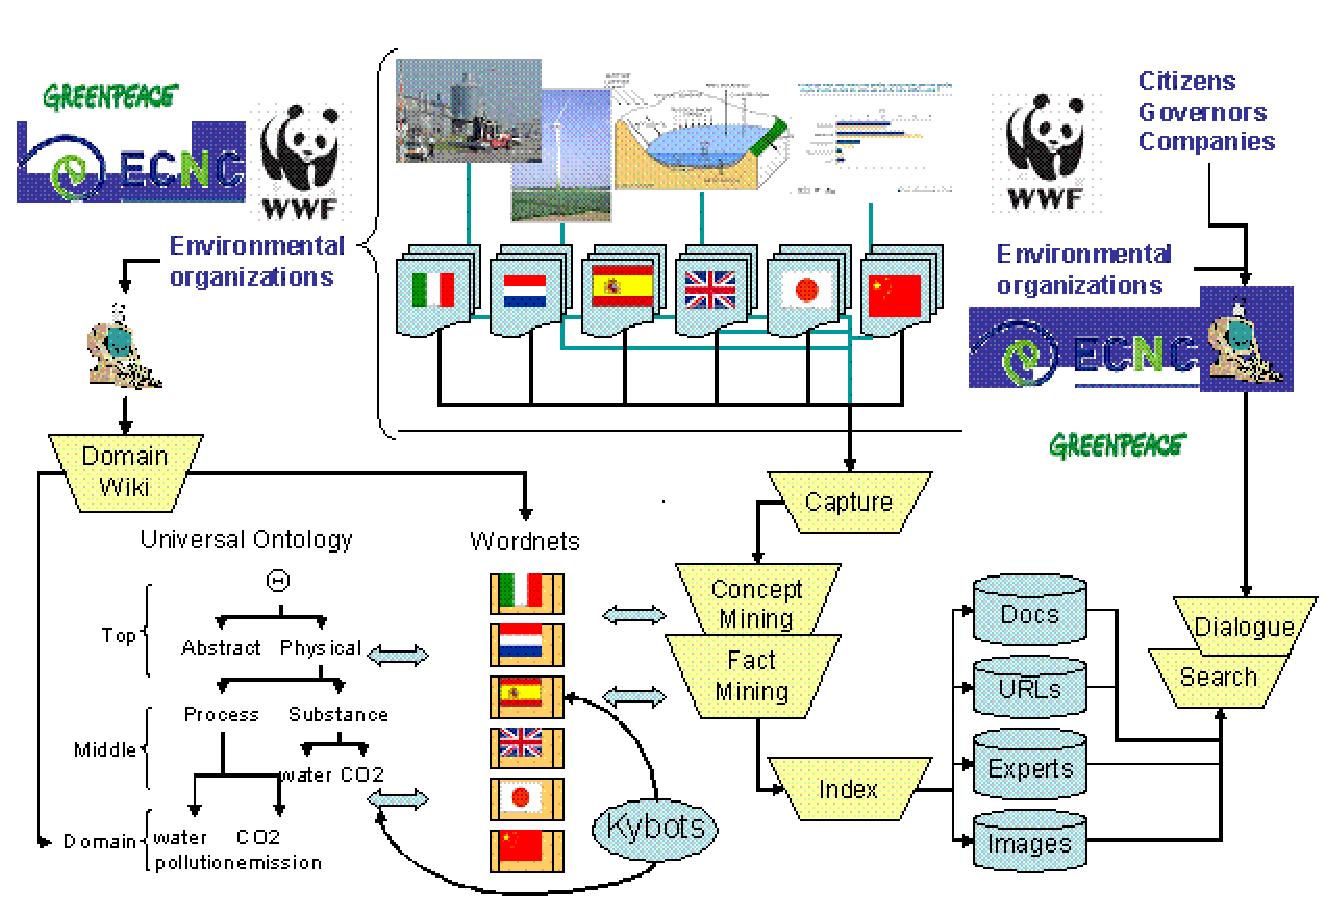
\includegraphics[width=0.8\textwidth]{pics/kyoto-project.eps}
% \end{center}

% \myslide{What can computers do?}
% \MyLogo{}
% \begin{itemize}
% \item[Q] \textit{Do birds migrate through Turkey?}
% \item[A] Yes.  \textit{The crane ($\subset$ bird) flies across Ankara ($\subset$ bird)}.
%   \begin{quote}
%     \large   fly$_1$ ($e_1$, crane$_5$($x_1$)),  across($e_2$,$e_1$,$x_2$), Ankara($x_2$).
%   \end{quote}
%   \begin{itemize}
%   \item  \textit{through} and \textit{across} are both \textit{path} roles.
%   \item \textit{fly} and \textit{migrate} are both \textit{motion} verbs.
%   \item Ankara is in Turkey
%   \end{itemize}
% \item Why do this?
%   \begin{itemize}
%   \item Local environmental knowledge often not translated into many languages
%   \item Facts may only occur in a few documents
% \end{itemize}
% \end{itemize}


\myslide{Information Structure}

\begin{itemize}
\item Many languages signal whether information is \txx{new} or \txx{given}

\item We can signal this in many ways:
  \begin{itemize}
  \item Determiners in English
  \item Intonation (focus)
  \item Topic marking
  \end{itemize}
\end{itemize}



\myslide{Cooperation in Conversation}
\begin{itemize}
\item \txx{Cooperative Principle}: people cooperate in conversation
  \begin{quote}
    ``Make your conversational contribution such as is required, at the stage at which it occurs, by the accepted purpose or direction of the talk exchange in which you are engaged.''
  \end{quote}
\item \txx{Implicature}
  \begin{quote}
    The aspect of meaning that a speaker conveys, implies, or suggests
    without directly expressing.
  \end{quote}
 \eng{Can you pass  the salt?} may implicate ``pass me the salt''
\end{itemize}

\myslide{Gricean Maxims}
\begin{small}
\begin{description}
\item [Maxim of Quantity] ~
  \begin{itemize}
  \item Make your contribution as informative as is required (for the current purposes of the exchange).
  \item Do not make your contribution more informative than is required.
  \end{itemize}
\item [Maxim of Quality] ~
  \begin{itemize}
  \item Do not say what you believe to be false.
  \item Do not say that for which you lack proper evidence.
  \end{itemize}
%\newpage
\item [Maxim of Relation] ~
  \begin{itemize}
  \item Be relevant.
  \end{itemize}
\item [Maxim of Manner] ~
  \begin{itemize}
  \item Be perspicuous [= be easily understood]
  \item Avoid obscurity of expression.
  \item Avoid ambiguity
  \item Be brief (avoid unnecessary prolixity)
  \item Be orderly
  \end{itemize}
\end{description}
\end{small}
\myslide{Conversational Implicatures and Hedges}
\begin{itemize}
\item \txx{Generalised conversational implicatures}
\\ the inferences we make by assuming cooperation
\item \txx{Particularised conversational implicatures}
\\ local inferences for a given situation
\item \txx{Scalar implicatures (Horn Scales)}
\\ one item on  a scale implicates all weaker items (and no stronger ones)
\item \txx{Conventional implicatures}
\\ implicatures attached to lexical items
\item \txx{Hedges}: show we know we are flouting a maxim
\end{itemize}


\section{Revision: \\ Speech as Action}


\myslide{Speech as Action}

\begin{itemize}
\item Language is often used to \emp{do} things: \txx{speech acts}
  \\ language has both
  \begin{itemize}
  \item \txx{interactivity}
  \item \txx{context dependence}
  \end{itemize}
\item There are four syntactic types that correlate closely to pragmatic uses

  \begin{tabular}{lcl}
  \txx{declarative}  &$\leftrightarrow$& \txx{assertion} \\
  \txx{interrogative} &$\leftrightarrow$& \txx{question} \\
  \txx{imperative} &$\leftrightarrow$& \txx{order} \\
  \txx{optative} &$\leftrightarrow$& \txx{wish}
  \end{tabular}
\item Mismatches between syntactic type and pragmatic use give rise to \\
  \txx{indirect speech acts}
\end{itemize}

\myslide{Perfomative Utterances}

\begin{exe}
  \ex \eng{I promise I won't drive home}
  \ex \eng{I bet you 5 bucks they get caught }
  \ex \eng{I declare this lecture over }
  \ex \eng{I warn you that legal action will ensue}
  \ex \eng{I name this ship \textit{the Lollipop} }
\end{exe}

\begin{itemize}
\item Uttering these (in an appropriate context) \emp{is} acting
\\  \emp{Utterances themselves can be actions}
\item In English, we can signal this explicitly with \textit{hereby}
\end{itemize}

\myslide{Felicity Conditions}
\begin{itemize}
\item Performatives (vs Constantives) \hfill (Austin)
\\ Given the correct \txx{felicity conditions}
  \begin{description}
  \item[A1] There must exist an accepted conventional procedure that
    includes saying certain words by certain persons in certain
    circumstances,
  \item[A2] The circumstances must be appropriate for the invocation
  \item[B1] All participants must do it both correctly
  \item[B2] \ldots  and completely
  \item[C1] The intention must be to do this the act
  \item[C2] The participants must conduct themselves so subsequently.
  \end{description}
\item If the conditions don't hold, the speech act is \txx{infelicitous}
  \begin{itemize}
  \item Failing \textbf{A} or \textbf{B} is a \txx{misfire}
  \item Failing \textbf{C} is an \txx{abuse}
  \end{itemize}
  \end{itemize}

\myslide{Explicit and Implicit Performatives}
\begin{itemize}
\item \txx{Explicit Performatives}
  \begin{itemize}
  \item Tend to be first person
  \item The main verb  is a performative: 
    \eng{promise, warn, sentence, bet, pronounce, \ldots}
  \item You can use \eng{hereby}
  \end{itemize}
\item \txx{Implicit Performatives}
  \begin{exe}
    \ex \eng{You are hereby charged with treason}
    \ex \eng{Students are requested to be quiet in the halls}
    \ex \eng{10 bucks says they'll be late}
    \ex \eng{Come up and see me some time! }
  \end{exe}
  Can be made explicit by adding a perfomative verb
\end{itemize}

\myslide{Elements of Speech Acts}
\begin{description}
\item \txx{Locutionary act} the act of saying something
\item \txx{\underline{Illocutionary act}} the force of the statement 
\item \txx{Perlocutionary act} the effects of the statement
\end{description}
Illocutionary force indicating devices(IFID)
\begin{itemize}
\item   word order;  stress;    intonation contour;  punctuation; the mood of the verb
 performative verbs: \eng{I (Vp) you that \ldots} 
\end{itemize}

\myslide{Searle's speech act classification}
  \begin{description}
  \item \txx{Declaration} changes the world (like performatives)
  \item \txx{Representative} describes the (speaker's view of the) world 
  \item \txx{Expressives}  express how the speaker feels
  \item \txx{Directives} get someone else to do something
  \item \txx{Commissives} commit oneself to a future action
  \end{description}


\myslide{Literal and non-literal uses}
\MyLogo{in indirect speech acts}
\begin{exe}
  \ex
  \begin{xlist}
    \ex \eng{Could you get that? }
    \ex \eng{Please answer the door.}
  \end{xlist}
  \ex 
  \begin{xlist}
    \ex \eng{I wish you wouldn't do that.}
    \ex \eng{Please don't do that.}
  \end{xlist}
  \ex
  \begin{xlist}
    \ex \eng{You left the door open.}
    \ex \eng{Please close the door.}
  \end{xlist}
\end{exe}
\begin{itemize}
\item People have access to both the literal and non-literal meanings
\item Non literal meanings can be slower to understand
\item Some non-literal uses are very conventionalized 
  \\ \eng{Can/Could you X?} \into \eng{Please X}
\item Questioning the felicity conditions produces an indirect version
\end{itemize}

\myslide{Felicity Conditions for Requesting}
\MyLogo{Searle (1969), simplified}
These things must hold for an utterance to be a \txx{request}:
\begin{itemize}
\item \textbf{Preparatory 1}: $H$ is able to perform  $A$
\item \textbf{Preparatory 2}: It is not obvious that the $H$ would perform $A$  without being asked
\item \textbf{Propositional:} $S$ predicates a future act $A$ of $H$
\item \textbf{Sincerity:}  $S$ wants $H$ to do $A$ 
\item \textbf{Essential:} The utterance $e$ counts as an attempt by $S$ to get $H$ to do $A$
\end{itemize}


 
\myslide{Why be Indirect?}

\begin{itemize}
\item Mainly for politeness
\begin{itemize}
\item \txx{Positive Face} desire to seem worthy and deserving of approval
\item \txx{Negative Face} desire to be autonomous, unimpeded by others
\item Threats to another’s face
  \begin{itemize}
  \item to positive: disapproval, disagreement, interruption
  \item to negative: orders, requests, suggestions
  \end{itemize}
\item Face-saving acts: 
  \begin{itemize}
  \item don't threaten another’s face: \eng{I may be wrong but, \ldots}
  \item allow for negative face: \eng{Could you please, \ldots}
  \end{itemize}
\item Is politeness trans-cultural?
\end{itemize}
\end{itemize}

\section{Revision: \\ Componential Analysis}


\myslide{Break word meaning into its components}
\begin{itemize} \addtolength{\itemsep}{-2ex}
\item components allow a compact description
\item interact with morphology/syntax
\item form part of our cognitive architecture
\item For example:
  \\[2ex] \begin{tabular}{lllll}
    \lex{woman} & \cmp{female} & \cmp{adult} & \cmp{human} & \\
    \lex{spinster} & \cmp{female} & \cmp{adult} & \cmp{human} & \cmp{unmarried} \\
    \lex{bachelor} & \cmp{male} & \cmp{adult} & \cmp{human} & \cmp{unmarried} \\
    \lex{wife} & \cmp{female} & \cmp{adult} & \cmp{human} & \cmp{married} \\
  \end{tabular}
\item We can make things more economical (fewer components):
  \\[2ex] \begin{tabular}{lllll}
    \lex{woman} & \cmp{+female} & \cmp{+adult} & \cmp{+human} & \\
    \lex{spinster} & \cmp{+female} & \cmp{+adult} & \cmp{+human} & \cmp{--married} \\
    \lex{bachelor} & \cmp{--female} & \cmp{+adult} & \cmp{+human} & \cmp{--married} \\
    \lex{wife} & \cmp{+female} & \cmp{+adult} & \cmp{+human} & \cmp{+married} \\
  \end{tabular}
\end{itemize}

\myslide{Defining Relations using Components}

\begin{itemize}
\item \txx{hyponymy}: 
    P is a hyponym of Q if all the components of Q are also in P.
\\ \lex{spinster} $\subset$ \lex{woman}; \lex{wife} $\subset$ \lex{woman}
\item \txx{incompatibility}:
    P is incompatible with Q if they share some
    components but differ in one or more \txx{contrasting} components
\\  \lex{spinster} $\not\approx$ \lex{wife}
\item{Redundancy Rules}
\\[2ex]  \begin{tabular}{llll}
     \cmp{+human} & \into & \cmp{+animate}  \\
     % \cmp{+adult} & \into & \cmp{+animate}  \\
      \cmp{+animate} & \into & \cmp{+concrete}  \\
     \cmp{+married} & \into & \cmp{+adult}  \\
     \cmp{+married} & \into & \cmp{+human}   & \ldots
  \end{tabular}
\end{itemize} 


\myslide{Katz’s Semantic Theory}

\begin{itemize}
\item Semantic rules must be recursive to deal with infinite meaning
\item Semantic rules interact with syntactic rule to build up meaning \txx{compositionally}
  \begin{itemize}
  \item A \txx{dictionary} pairs lexical items with semantic representations
 \begin{itemize}
 \item (\txx{semantic markers}) are the links that bind lexical items
   together in lexical relations
 \item {[\txx{distinguishers}]} serve to identify this particular lexical item
   \\ this information is not relevant to syntax
 \end{itemize}
\item\txx{projection rules} show how meaning is built up
  \begin{itemize}
  \item Information is passed up the tree and collected at the top.
  \item \txx{Selectional restrictions} help to reduce ambiguity and
    limit the possible readings
  \end{itemize}
\end{itemize}

  
\myslide{Verb Classification}
\MyLogo{Levin (1993)}

\begin{itemize}
\item We can investigate the meaning of a verb by looking at its
  grammatical behavior
  \begin{exe}
    \ex Consider the following transitive verbs
    \begin{xlist}
      \ex \eng{Margaret \ul{cut} the bread}
      \ex \eng{Janet \ul{broke} the vase}
      \ex \eng{Terry \ul{touched} the cat}
      \ex \eng{Carla \ul{hit} the door}
    \end{xlist}
  \end{exe}
\item These do not all allow the same argument structure alternations

\end{itemize}
\myslide{Diathesis Alternations}

\begin{itemize}
\item \txx{Causative/inchoative} alternation:
  \begin{quote}
    \eng{Kim \ul{broke} the window} $\leftrightarrow$ \eng{The window \ul{broke}}
    \\ also \eng{the window \ul{is broken}} (state)
  \end{quote}
\item \txx{Middle construction} alternation:
  \begin{quote}
    \eng{Kim \ul{cut} the bread} $\leftrightarrow$ \eng{The bread \ul{cut} easily}
  \end{quote}
\item \txx{Conative} alternation:
  \begin{quote}
    \eng{Kim \ul{hit} the door} $\leftrightarrow$ \eng{Kim \ul{hit} at the door}
  \end{quote}
\item \txx{Body-part possessor ascension} alternation:
  \begin{quote}
    \eng{Kim \ul{cut} Sandy's arm} $\leftrightarrow$ 
    \eng{Kim \ul{cut} Sandy on the arm}
  \end{quote}
\end{itemize}




\myslide{Diathesis Alternations and Verb Classes}

\MyLogo{Levin (1993)}

\begin{itemize}
\item A verb's (in)compatibility with different alternations is a strong
  predictor of its lexical semantics:
  \begin{quote}\smaller[1]
    \begin{tabular}{lcccc}
      & \lex{break} & \lex{cut} & \lex{hit} & \lex{touch} \\
      Causative & YES & NO & NO & NO \\
      Middle & YES & YES & NO & NO \\
      Conative & NO & YES & YES & NO \\
      Body-part & NO & YES & YES & YES \\
    \end{tabular}
    \vspace{3ex}
  \end{quote}

\item We can analyze components that correlate with the alternations
  \\[2ex]
  \begin{tabular}{lll}
  \lex{break} & \textsc{cause, change} & 
  \{\eng{break, chip, crack, crash, crush, ...}\}\\
  \lex{cut}   & \textsc{cause, change, }& 
  \{\eng{chip, clip, cut, hack, hew, saw, ...}\}\\ 
   & \textsc{contact, motion} \\
  \lex{hit}   & \textsc{contact, motion}&
  \{\eng{bang, bash, batter, beat, bump, ...}\}\\
  \lex{touch} & \textsc{contact}&
 \{\eng{caress, graze, kiss, lick, nudge, ...}\}
  \end{tabular}

\end{itemize}

\myslide{Cognitive Semantics}
\MyLogo{Talmy (1975, 1983, 1985, 2000)}
\begin{itemize}
\item Major semantic components of Motion:
\begin{itemize}
\item \txx{Figure}: object moving or located with respect to the \txx{ground} 
\item \txx{Ground}: reference object
\item \txx{Motion}: the presence of movement of location in the event
\item \txx{Path}: the course followed or site occupied by the Figure
\item \txx{Manner}: the type of motion
\end{itemize}
\begin{exe}
  \ex \gll Kim swam {away from} {the crocodile} \\
  Figure Manner Path Ground \\
  \ex \gll {The banana} hung from {the tree} \\
  Figure Manner Path Ground \\
\end{exe}
\item These are lexicalized differently in different languages.
\\ \begin{tabular}{ll}
  Language (Family) & Verb Conflation Pattern \\ \hline
  Romance, Semitic, Polynesian, \ldots & Path + fact-of-Motion \\
  Indo-European ($-$ Romance), Chinese & Manner/Cause + fact-of-Motion \\
  Navajo, Atsuwegei, \ldots & Figure + fact-of-Motion 
\end{tabular}
\end{itemize}

\myslide{Jackendoff’s Lexical Conceptual Structure} 

\begin{itemize}
\item An attempt to explain how we think
\item \txx{Mentalist Postulate}
  \begin{quote}
    Meaning in natural language is an information structure that is
    mentally encoded by human beings
  \end{quote}
\item Universal Semantic Categories
  \begin{itemize}
  \item \txx{Event}
  \item \txx{State}
  \item \txx{Material Thing/Object}
  \item \txx{Path}
  \item \txx{Place}
  \item \txx{Property}
  \end{itemize}
\end{itemize}

\myslide{Motion as a tree}

\begin{multicols}{2}
  \begin{exe}
    \ex \eng{Bobby went into the house}
    \ex ``Bobby traverses a path that terminates at the interior of the house''
    \ex
    \begin{tree}
      \br{Event}{\lf{GO}
        \br{Thing}{ \lf{BOBBY}}
        \br{Path}{\lf{TO}
          \br{Place}{\lf{IN}\br{Thing}{\lf{HOUSE}}}}}
    \end{tree}
    %\newpage
    \ex \eng{The car is in the garage}
    \ex ``The car is in the state located in the interior of the garage''
    \ex
    \begin{tree}
      \br{State}{\lf{BE-LOC}
        \br{Thing}{ \lf{CAR}}
        \br{Place}{\lf{IN}\br{Thing}{\lf{GARAGE}}}}
    \end{tree}
\end{exe}
\end{multicols}


\myslide{Things: Boundedness and Internal Structure}
\begin{itemize}
\item Two components:
\\[2ex]  \begin{tabular}{llll}
    Boundedness & Internal Struct. & Type & Example\\ \hline
    $+$b & $-$i & \txx{individuals} & \eng{a dog}/\eng{two dogs}\\
    $+$b & $+$i & \txx{groups}      & \eng{a committee}\\
    $-$b & $-$i & \txx{substance}s  & \eng{water}\\
    $-$b & $+$i & \txx{aggregates}  & \eng{buses, cattle}
  \end{tabular}

\item This can be extended to verb aspect (the verb event is also [$\pm$b, $\pm$i]).
  \\ \lex{sleep} [$-$b], \lex{cough} [$+$b], \lex{eat}  [$\pm$b]
 \begin{exe}
   \ex Bill ate two hot dogs in two hours.
   \ex *Bill ate hot dogs in two hours.
   \ex $^\#$Bill ate two hot dogs for two hours.
   \ex Bill ate hot dogs for two hours.
\end{exe}
\end{itemize}

\myslide{Conversion: Boundedness and Internal Structure}
\MyLogo{See Bond (2005) for an extension to Japanese and computational implementation.}
\begin{itemize}
\item Including
 \\[2ex] \begin{tabular}{lll}
  \txx{plural} & {[+b, --i] \into\ [--b, +i]} &     
    \eng{brick}  \into\ \eng{bricks} \\
  \txx{composed of} &{[--b, +i] \into\ [+b, --i]} &
     \eng{bricks}  \into\ \eng{house of bricks} \\
  \txx{containing} &   {[--b, --i] \into\ [+b, --i]} &
     \eng{coffee}  \into\ \eng{a cup of coffee/a coffee}
  \end{tabular}
\bigskip\bigskip\bigskip
\item Excluding
  \\[2ex] \begin{tabular}{lll}
    \txx{element}  & {[--b,+i] \into\ [+b, --i]} &     
    \eng{grain of rice} \\
    \txx{partitive} & {[--b, $\pm$i] \into\ [+b, --i]} &     
    \eng{top of the mountain}, \eng{one of the dogs} \\
    \txx{universal grinder} &  {[+b, --i] \into\ [--b, --i]} &     
    \eng{There's \ul{dog} all over the road}
  \end{tabular}
\end{itemize}



\myslide{Pustejovsky’s Generative Lexicon}
\MyLogo{}

\begin{itemize} 
\item Each lexical entry can have:\\
  \textsc{argument structure}\\
  \textsc{event structure}\\
  \textsc{lexical  inheritance structure}\\
  \textsc{qualia structure}:\\
  \begin{tabular}{ll}
    \textsc{constitutive} & constituent parts \\
    \textsc{formal} & relation to other things \\
    \textsc{telic} & purpose \\
    \textsc{agentive}  & how it is made
  \end{tabular}
\item Interpretation is \txx{generated} by combing word meanings
\item Events have \textbf{complex} structure
 \\ \begin{tabular}{ccc}
    \txx{State}  & \txx{Process} & \txx{Transition} \\
 \begin{tree}
    \br{S}{\lf{e}}
  \end{tree}
  &    \begin{tree}
    \br{P}{\tlf{e$_1$ \ldots e$_n$}}
  \end{tree}
  &     \begin{tree}
    \br{T}{\lf{E$_1$} \lf{$\neg$ E$_2$}}
  \end{tree}
  \\   \lex{understand, love, be tall}
  &    \lex{sing, walk, swim}
  &     \lex{open, close, build}
\end{tabular}
\end{itemize}
\end{itemize}

% \myslide{Different Alternations}
%   \begin{exe}
%     \ex \eng{The door closed}
%    \begin{tree}
%       \br{T}{\br{P}{\br{[$\neg$ closed(door)]}{}}
%         \br{S}{\br{[closed(door)]}{}}} 
%     \end{tree}
%     \ex \eng{Jamie closed the door}
%     \begin{tree}
%       \br{T}{\br{P}{\br{[act(j, door) $\wedge$ $\neg$ closed(door)]}{}}
%         \br{S}{\br{[closed(door)]}{}}} 
%     \end{tree}
%     \ex \eng{The door is closed}
%    \begin{tree}
%       \br{S}{\br{e}{\br{[closed(door)]}{}}}
%     \end{tree}
%   \end{exe}

\myslide{Modifier Ambiguity}
\MyLogo{}
  \begin{exe}
    \ex \eng{Jamie closed the door rudely}
    \ex \eng{Jamie closed the door in a rude way [with his foot]}
    \\\begin{tree}
      \br{T}{\br{P [rude(P)]}{\br{[act(j, door) $\wedge$ $\neg$ closed(door)]}{}}
        \br{S}{\br{[closed(door)]}{}}} 
    \end{tree}
    \ex \eng{It was rude of Jamie to close the door}
    \\\begin{tree}
      \br{T [rude(T)]}{\br{P}{\br{[act(j, door) $\wedge$ $\neg$ closed(door)]}{}}
        \br{S}{\br{[closed(door)]}{}}} 
    \end{tree}
  \end{exe}

\myslide{Qualia Structure}
\MyLogo{}

\begin{exe}
  \ex \eng{fast typist}
  \begin{xlist}
    \ex\label{ta} a typist who is fast [at running]
    \ex\label{tb} a typist who types fast
  \end{xlist}
%  \ex \eng{Joan baked the potato}
\end{exe}
\begin{itemize}
\item typist 
 \begin{avm} \[
    \textsc{argstr} &
    \[
      \textsc{arg1} & \iz{x:typist}\\
    \]\\
    \textsc{qualia} &
    \[
      \textsc{formal} & \[ \iz{x}  [ $\subset$ \iz{person} ]\] \\
      \textsc{telic} & \[ \iz{type(e,x)}  \]
      \] 
 \]
\end{avm}
\item (\ref{ta}) \eng{fast} modifies $x$
\item (\ref{tb}) \eng{fast} modifies $e$
\end{itemize}



\myslide{Summary}

\begin{itemize}
\item Meaning can be broken up into units smaller than words:  \txx{components} 
  \begin{itemize}
  \item These can be combined to make larger meanings
  \item At least some of them influence syntax
  \item They may be psychologically real
  \end{itemize}
\item Problems with Components of Meaning
  \begin{itemize}
  \item Primitives are no different from necessary and sufficient conditions
    \\ it is impossible to agree on the definitions
    \\ but they allow us to state generalizations better
  \item Psycho-linguistic evidence is weak
  \item It is just \txx{markerese}
  \item There is no \txx{grounding}
  \end{itemize}
\end{itemize}

\section{Revision: Formal Semantics}

\myslide{Language meets Logic (again)}

\begin{itemize}
\item \txx{formal semantics} is also known as
  \begin{itemize}
  \item \txx{truth-conditional semantics}
  \item \txx{model-theoretic semantics}
  \item \txx{Montague Grammar}
  \item \txx{logical semantics}
  \end{itemize}
\item A general attempt to link the meaning of sentences to the
  circumstances of the world: \txx{correspondence theory}
  \begin{itemize}
  \item If the meaning of the sentence and the state of the world
    \emp{correspond} then the sentence is \textbf{true}
  \end{itemize}
\end{itemize}

\myslide{Model-Theoretical Semantics}

\begin{enumerate}
\item Translate from a natural language into a logical language
  with explicitly defined syntax and semantics
\item Establish a mathematical model of the situations that the
  language describes
\item Establish procedures for checking the mapping between the
  expressions in the logical language and the modeled situations.
\end{enumerate}


\myslide{Translating English into a Logical Metalanguage}
%\myslide{Empirical truths and connectives}
\MyLogo{Recall lecture 4}
\begin{itemize}
\item Consider simple sentences
  \begin{itemize}
  \item Represent the predicates by a capital \txx{predicate letter}
    \\ these can be n-ary
  \item Represent the \txx{individual constants} by lower case letters
  \item Represent \txx{variables} by lower case letters (x,y,z)
  \end{itemize}
\item Join simple sentences with logical connectives
\\ treat relative clauses as \txx{and}
  \begin{exe}
    \ex \eng{Bobbie who is asleep writhes}: A(b) $\wedge$ W(b)
    \ex \eng{Bobbie is asleep and Freddie drinks}: A(b) $\wedge$ D(f)
    \ex \eng{Freddie drinks and sleeps}: D(f) $\wedge$ S(f)
    \ex \eng{Freddie doesn't drink beer}: $\neg$ D(f,b)
    \ex \eng{If Freddie drinks whiskey Bobbie sleeps}: D(f,w) \into S(b)
%    \ex \eng{x is asleep}: A(x)
  \end{exe}
\end{itemize}

\myslide{Quantifiers in Predicate Logic}
\MyLogo{$\forall$ and \into; $\exists$ and $\wedge$}

\begin{itemize}
  \item Quantifiers bind variables and scope over predications
    \begin{itemize}
    \item \txx{Universal Quantifier} ($\forall$: \eng{each, every, all})
    \item \txx{Existential Quantifier} ($\exists$: \eng{some, a})
    \end{itemize}
    \begin{exe}
      \ex \eng{All students learn logic}: $\forall$x (S(x)  $\into$ L(x,l))
      \ex \eng{A student learns logic}: $\exists$x (S(x)  $\wedge$ L(x,l))
      \ex \eng{Some students learn logic}: $\exists$x (S(x)  $\wedge$ L(x,l))
      \ex \eng{No students learn logic}: $\neg\exists$x (S(x)  $\wedge$ L(x,l))
      \ex \eng{All students don't learn logic}: $\forall$x (S(x)  $\into$ $\neg$L(x,l))
    \end{exe}
  \item All variables must be bound
\end{itemize}

\myslide{Some Advantages in Translating to Predicate Logic}
\MyLogo{}

\begin{itemize}
\item Explicit representation of scope ambiguity
  \begin{exe}
    \ex \eng{Everyone loves someone}
    \begin{xlist}
          \ex \eng{Everyone has someone they love}:  $\forall$x$\exists$y (L(x,y))
          \ex \eng{There is some person who is loved by everyone}: 
          $\exists$y$\forall$x (L(x,y))
    \end{xlist}
  \end{exe}
\item But the big advantage is in reasoning with the real world
   \\ \txx{denotational semantic analysis}
\end{itemize}


\myslide{Creating a \txx{Model}}

\begin{enumerate}\addtolength{\itemsep}{-1.5ex}
\item a \txx{semantic interpretation} of the symbols of the predicate logic
\item a \txx{domain}: the model of a situation which identifies the
  linguistically relevant entities, properties and relations
\item a \txx{denotation assignment function}: this is a procedure
  which matches the linguistic elements with the items  that they denote (a \txx{naming function})
\end{enumerate}
\begin{itemize}
\item Is the denotation correct (does it match the real world)?
  \begin{itemize}
  \item \textbf{Sentence} 
    $p$ is true in situation $v$ if it corresponds with the real world: 
    \\ {[$p$]$^v$ = 1}: the denotatum of $p$ in $v$ is true
  \item \textbf{Constant} denotation of a constant is the individual entity in question
  \item \textbf{Predicate constants} are sets of individuals for which the predicate holds
\\ {\{$<x, y, z>$: $x$ hands $y$ to $z$\}}
  \end{itemize}

\end{itemize}

% \myslide{The Domain}

% \begin{itemize}
% \item The domain represents the individuals and representations in a situation $v$
% \item Combine this with an assignment function $F$ to form a model
% \\ $M_1 = <U_1, F_1>$ (or set of models: $M_2 = <U_1, F_2>$, \ldots)
% \end{itemize}

% \myslide{Evaluating a simple statement}
% \begin{itemize}
% \item How can we check if \eng{Ian sings},   S(i), is true?
%   \begin{itemize}
%   \item {[S(i)]$^{M_1}$ = 1 iff [i]$^{M_1} \in$ [S]$^{M_1}$} \\ The
%     sentence is true if and only if the extension of \eng{Ian} is part of
%     the set defined by \eng{sings} in the model $M_1$
%   \item $F_1$(i) = Ian; $F_1$(S) =   \{Ian, Peter\};  Ian $\in$  \{Ian, Peter\}
%   \item[$\Rightarrow$] [S(i)]$^{M_1}$ = 1
%   \end{itemize}
% \item \eng{Did Martin produce everyone in Joy Division}
%   \begin{itemize}
%   \item $\forall$x (J(x) $\wedge$ O(m,x))
%     \begin{itemize}
%     \item i $\wedge$ O(m,i) = ?; b $\wedge$ O(m,b) = ?;  p $\wedge$ O(m,p) = ?;
%       s $\wedge$ O(m,s) = ?
%     \end{itemize}
%   \item 1,1,1,1  = ?
%   \item[$\Rightarrow$] [$\forall$x (J(x) $\wedge$ O(m,x))] = 1  \hfill Yes
%   \end{itemize}
% \end{itemize}


\myslide{Defining Relations using Logic}

\begin{itemize}
\item \txx{hyponymy}
  \begin{itemize}
  \item $\forall$x(DOG(x) \into\ ANIMAL(x))
  \end{itemize}
\item \txx{antonym}
  \begin{itemize}
  \item $\forall$x(DEAD(x) \into\ $\neg$ALIVE(x))
  \end{itemize}
\item \txx{converse}
  \begin{itemize}
  \item $\forall$x$\forall$y(PARENT(x,y) \into\ CHILD(y,x))
  \end{itemize}
\item \txx{synonym}
  \begin{itemize}
  \item $\forall$x((EGGPLANT(x) \into\ BRINJAL(x)) $\wedge$ 
    (BRINJAL(x) \into EGGPLANT(x)))
  \end{itemize}
\end{itemize}



\myslide{Restricted Quantifiers}

\begin{itemize}
\item \eng{Most students read a book}
  \begin{itemize}
  \item Most(x)(S(x) $\wedge$ R(x))
    \\ \eng{most things are students and most things read books}
  \item Most(x)(S(x) iff R(x))
    \\ \eng{most things, if they are students, read books}
  \end{itemize}
\item We need to restrict the quantification
  \begin{itemize}
  \item (Most x: S(x)) R(x)
  \end{itemize}
\item Sometimes we need to decompose
  \begin{itemize}
  \item \eng{everybody} ($\forall$x: P(x))
  \item \eng{something} ($\exists$x: T(x))
  \end{itemize}
\end{itemize}

\myslide{Higher Order Logic}
 \begin{itemize}
\item Recall  \eng{Ian sings}
  \begin{itemize}
  \item {[S(i)]$^{M_1}$ = 1 iff [i]$^{M_1} \in$ [S]$^{M_1}$} \\ The
    sentence is true if and only if the extension of \eng{Ian} is part of
    the set defined by \eng{sings} in the model $M_1$
  \item Remodel, with sing a property of Ian: i(S) \\ {[i(S)]$^{M_1}$
      = 1 iff [S]$^{M_1} \in$ [i]$^{M_1}$} \\ The sentence is true if
    and only if the denotation of the verb phrase \textit{sings} is
    part of the extension of \eng{Ian}  in the model $M_1$
  \end{itemize}
\item \eng{Ian} is a set of sets of properties: \txx{second-order logic}
\end{itemize}

\myslide{Generalized Quantifiers} 

\begin{itemize}
\item Q(A,B): \eng{Q A are B}
\item most(A,B) =1 iff $|$ A $\cap$ B $| > |$ A $-$ B $|$ 
\item all(A,B) =1 iff  A $\subseteq$ B  
\item some(A,B) =1 iff  A $\cap$ B $\ne \emptyset$ 
\item no(A,B) =1 iff A $\cap$ B  $= \emptyset$ 
\item fewer than x(A,B,X) =1 iff $|$ A $\cap$ B $| <  |$ X $|$ 
\end{itemize}

\myslide{Strong/Weak Quantifiers}

\begin{exe}
  \ex only \txx{weak} quantifiers can occur in existential \eng{there} sentences
  \begin{xlist}
    \ex \eng{There is a fox in the henhouse}
    \ex \eng{There are two foxes in the henhouse}
    \ex \eng{*There is every fox in the henhouse}
    \ex \eng{*There are both foxes in the henhouse}
  \end{xlist}
\end{exe}
\begin{itemize}
\item \txx{symmetrical} (cardinal) quantifiers are \txx{weak}
  \\ det(A,B) = det(B,A)
  \begin{exe}
    \ex \eng{three lecturers are Australian}   = \eng{three Australians are lecturers}
  \end{exe}
\item \txx{asymmetrical} (cardinal) quantifiers are \txx{strong}
  \\ det(A,B) $\ne$ det(B,A)
  \begin{exe}
    \ex \eng{both lecturers are Australian}   = \eng{both Australians are lecturers}
  \end{exe}

\end{itemize}

\myslide{Negative Polarity Items}

\begin{itemize}
\item Some words in English appear only in downward entailing expressions
  \begin{itemize}
  \item \txx{Upward entailment} goes from a subset to a set
  \item \txx{Downward entailment} goes from a set to a subset
  \end{itemize}
\end{itemize}
\begin{exe}
  \ex
  \begin{xlist}
    \ex \eng{Kim does\ull{n't} eat dessert} \ent  \eng{Kim does\ull{n't} eat hot dessert}
    \ex \eng{Kim does\ull{n't} eat hot dessert} \nent  \eng{Kim does\ull{n't} eat dessert}
    \trans \textbf{Downward entailment}
    \end{xlist}
    \ex
  \begin{xlist}
    \ex \eng{Kim eats some desserts} \nent  \eng{Kim eats hot dessert}
    \ex \eng{Kim eats some hot dessert} \ent  \eng{Kim  eats some desserts}
    \trans \textbf{Upward entailment}
    \end{xlist}
  \end{exe}
  \begin{itemize}
  \item Negative Polarity Items are licensed by downward entailing expressions
  \end{itemize}


\myslide{Left and Right Monotonicity}

\begin{itemize}
\item The monotonicity may depend on the position
  \begin{exe}
    \ex 
 \begin{xlist}
    \ex \eng{Every student studies semantics} \nent  
    \eng{Every student studies formal semantics}
    \ex \eng{Every student studies formal semantics} \ent  
    \eng{Every student studies semantics}
    \trans \textbf{Upward entailment (right argument)}
    \end{xlist}
    \ex 
 \begin{xlist}
    \ex \eng{Every student studies semantics} \ent  
    \eng{Every linguistics student studies  semantics}
    \ex \eng{Every linguistic student studies  semantics} \nent  
    \eng{Every student studies semantics}
    \trans \textbf{Downward entailment (left argument)}
    \end{xlist}
\newpage
  \ex 
 \begin{xlist}
    \ex \eng{Every student who has ever studied semantics loves it}
    \ex *\eng{Every student who has studied semantics ever loves it}
    \ex \eng{Few students who have ever studied semantics dislike it}
    \ex \eng{Few students who have studied semantics ever dislike it}
    \end{xlist}
  \end{exe}
\end{itemize}
\begin{itemize}
\item Formal models of quantification can be used to make predictions
  about seemingly unrelated phenomena
\end{itemize}

\myslide{More Examples}
 \begin{exe}
    \ex 
 \begin{xlist}
   \ex \eng{Every student is Italian.} \nent \eng{Every student is Italian and blond.}
   \ex \eng{Every student is Italian and blond.} \ent \eng{Every student is Italian.}
 \end{xlist}
 \ex 
 \begin{xlist}
   \ex \eng{Some student smokes.} \nent  \eng{Some Italian student smokes.}
   \ex \eng{Some Italian student smokes.} \ent \eng{Some student smokes.}
 \end{xlist}
 \ex 
 \begin{xlist}
\ex    \eng{Some student is Italian.}  \ent \eng{Some student is Italian and blond.}
\ex    \eng{Some student is Italian and blond.} \ent \eng{Some student is Italian.}
 \end{xlist}
 \ex 
 \begin{xlist}
   \ex \eng{No student smokes.} \ent \eng{No Italian student smokes.}
\ex    \eng{No Italian student smokes.} \nent \eng{No student smokes.}
 \end{xlist}
 \ex 
 \begin{xlist}
   \ex \eng{No student is Italian.}  \ent \eng{No student is Italian and blond.}
   \ex \eng{No student is Italian and blond.} \nent \eng{No student is Italian.}
 \end{xlist}
\end{exe}

With \lex{some} we must always infer from a more specific to a less
specific phrase (upward entailing). With \lex{no}, it's the opposite
%%% http://www.mamori.com/semantics/0507.pdf

% (7)
% a.
% Right upward entail
% ment
% D(A)(B
% 
% C)
% 
% D(A)(B)
% Some student is Italian and blond.
% 
% Some student is Italian.
% b.
% Ri
% ght downward entail
% ment
% D(A)(B)
% 
% D(A)(B
% 
% C)
% No students are Italian.
% 
% No students are Italian and blond.
% c.
% Left upward
% entail
% ment
% D(B
% 
% C)(A)
% 
% D(B)(A)
% Some Italian student smokes.
% 
% Some student
% smokes
% .
% d.
% Left downward entail
% ment
% D(B)(A)
% 
% D(B
% 
% C)(A)
% No students smoke.
% 
% No Italian students smoke.
% In sum,
% Some
% is upward entailing in its both arguments.
% No
% is downward entailing in its both arguments.
% Every
% is
% ...
% Few
% is
% ...
% So why
% do
% these entailment patterns matter?
% Distribution of negative polarity items
% (
% any, give a
% damn, ever
% , etc.)
% (
% 8
% )
% a.
% *John saw
% any
% bird.
% b.
% John did not see
% any
% bird.
% (
% 9
% )
% a.
% *Some student
% gives a damn
% about Pavarotti.
% b.
% *
% Every student
% gives a damn
% about Pavarotti.
% c.
% No student
% gives a damn
% about Pavarotti.
% (
% 10
% )
% a.
% *
% Some
% student
% have
% ever
% read a book about Pavarotti.
% b.
% *
% Every student has
% ever
% read a book about Pavarotti.
% c.
% No
% student ha
% s
% ever
% read a book about Pavarotti.
% (
% 11
% )
% a.
% *Some student who has
% ever
% read a book about Pavarotti would want to meet
% him.
% b.
% Every student
% who has
% ever
% read a book about Pavarotti would want to meet him.
% c. No student who has
% ever
% read a book about Pavarotti would want to meet him.
% When are
% negative polarity items
% licensed?
% Negatives, yes, but not only that (consider
% every
% in (
% 11
% b

% (7)
% a.
% Right upward entail
% ment
% D(A)(B
% 
% C)
% 
% D(A)(B)
% Some student is Italian and blond.
% 
% Some student is Italian.
% b.
% Ri
% ght downward entail
% ment
% D(A)(B)
% 
% D(A)(B
% 
% C)
% No students are Italian.
% 
% No students are Italian and blond.
% c.
% Left upward
% entail
% ment
% D(B
% 
% C)(A)
% 
% D(B)(A)
% Some Italian student smokes.
% 
% Some student
% smokes
% .
% d.
% Left downward entail
% ment
% D(B)(A)
% 
% D(B
% 
% C)(A)
% No students smoke.
% 
% No Italian students smoke.
% In sum,
% Some
% is upward entailing in its both arguments.
% No
% is downward entailing in its both arguments.
% Every
% is
% ...
% Few
% is
% ...
% So why
% do
% these entailment patterns matter?
% Distribution of negative polarity items
% (
% any, give a
% damn, ever
% , etc.)
% (
% 8
% )
% a.
% *John saw
% any
% bird.
% b.
% John did not see
% any
% bird.
% (
% 9
% )
% a.
% *Some student
% gives a damn
% about Pavarotti.
% b.
% *
% Every student
% gives a damn
% about Pavarotti.
% c.
% No student
% gives a damn
% about Pavarotti.
% (
% 10
% )
% a.
% *
% Some
% student
% have
% ever
% read a book about Pavarotti.
% b.
% *
% Every student has
% ever
% read a book about Pavarotti.
% c.
% No
% student ha
% s
% ever
% read a book about Pavarotti.
% (
% 11
% )
% a.
% *Some student who has
% ever
% read a book about Pavarotti would want to meet
% him.
% b.
% Every student
% who has
% ever
% read a book about Pavarotti would want to meet him.
% c. No student who has
% ever
% read a book about Pavarotti would want to meet him.
% When are
% negative polarity items
% licensed?
% Negatives, yes, but not only that (consider
% every
% in (
% 11
% b
% 3
% If we consider
% the
% directional entailing properties discussed above, a negative polarity item is
% licensed in a downward entailing environment.
% (Ladusaw 1979
% )
% What happens with
% not every
% ?
% (
% 10
% )
% b
% ’
% . Not every student has
% ever
% read a book about Pavarotti.
% (
% 11
% )
% b
% ’
% . Not every student who has
% ever
% read a book about Pavarotti would want to meet him.


\myslide{Anaphora}

\begin{exe}
  \ex 
  \begin{xlist}
    \ex \eng{R2D2$_i$ mistrusts itself$_i$}
    \ex M(r,r)
  \end{xlist}
 \ex 
  \begin{xlist}
    \ex \eng{Every robot mistrusts itself}
    \ex ($\forall$x: R(x)) M(x,x)
  \end{xlist}
 \ex 
  \begin{xlist}
    \ex \eng{Luke bought a robot and it doesn't work}
    \ex ($\exists$x: R(x)) B(l,x) $\wedge$ $\neg$W(x)
  \end{xlist}
 \ex 
  \begin{xlist}
    \ex \eng{Every robot went to Naboo.  ?It met Jar Jar.}
    \ex ($\forall$x: R(x)) W(x,n); M(x,j)\hfill \emp{unbound}
  \end{xlist}
 \ex 
  \begin{xlist}
    \ex \eng{A robot went to Naboo.  It met Jar Jar.}
    \ex ($\exists$x: R(x)) W(x,n); M(x,j)\hfill \emp{???}
  \end{xlist}
  \trans indefinite nominals exist beyond the sentence: \txx{discourse referents}
\ex 
  \begin{xlist}
    \ex \eng{Luke didn't buy a robot.  ?It met Jar Jar.}
  \end{xlist}
  \trans indefinite nominals scope can still be limited
\end{exe}

% \myslide{Donkey Sentences}

% \begin{exe}
%   \ex 
%   \begin{xlist}
%     \ex \eng{If R2D2$_i$ owns a ship it is rich}
%     \ex ($\exists$x (S(x) $\wedge$ O(r,x))) \into\ R(x)
%   \end{xlist}
%   \ex 
%   \begin{xlist}
%     \ex \eng{If a robot owns a ship it races it}
%     \ex *($\exists$x$\exists$y (R(x) $\wedge$ S(y) $\wedge$ O(x,y))) \into\ R(x,y)
%     \ex $\forall$x$\forall$y ((R(x) $\wedge$ S(y) $\wedge$ O(x,y)) \into\ R(x,y)
%   \end{xlist}
%   \trans $\exists$ needs to become $\forall$
%   \ex \eng{Every farmer who owns a donkey beats it}
% \end{exe}

% \myslide{Discourse Representation Theory}
% \begin{itemize}
% \item Build up Discourse Representation Structures
% \end{itemize}

% \begin{exe}
%    \ex 
%   \begin{xlist}
%     \ex \eng{Alex met a robot$_i$}
%     \ex \eng{It$_i$ smiled}
%   \end{xlist}
%   \ex \fbox{\begin{tabular}{l}
%       \cen{1}{x y} \\[2ex]
%     Alex(x) \\
%     robot(y) \\
%     met (x,y) 
%   \end{tabular}} 
% \hspace{5em} \fbox{\begin{tabular}{l}
%       \cen{1}{x y} \\[2ex]
%     Alex(x) \\
%     robot(y) \\
%     met (x,y) \\
%     u = y \\
%     smiled(u)
%   \end{tabular}}
% \end{exe}

% \myslide{Negative Contexts}

% \begin{exe}
%    \ex 
%   \begin{xlist}
%     \ex \eng{Luke does not own a robot}
%   \end{xlist}
%   \ex 
%   \fbox{\begin{tabular}{l}
%       \cen{1}{x} \\
%       Luke(x) \\
%       $\neg$\ \  \fbox{\begin{tabular}{l}
%           \cen{1}{y} \\[2ex]
%           robot(y) \\
%           own (x,y) 
%         \end{tabular}} 
%     \end{tabular}}
%   \end{exe}
%   \begin{itemize}
%   \item The contained DRS is \txx{subordinate}
%     \begin{itemize}
%     \item indefinite NPs in negated subordinate structures are inaccessible
%     \item names (constants) are always accessible
%     \end{itemize}
%   \end{itemize}

% % \myslide{Conditionals}

% % \begin{exe}
% %    \ex 
% %   \begin{xlist}
% %     \ex \eng{If Jo owns a robot then they are rich}
% %   \end{xlist}
% %   \ex 
% %   \fbox{\begin{tabular}{lll}
% %       & \cen{1}{x} \\
% %  \fbox{\begin{tabular}{l}
% %           \cen{1}{y} \\[2ex]
% %           Jo(x) \\
% %           robot(y) \\
% %           own (x,y) 
% %         \end{tabular}} 
% % & \into &
% %  \fbox{\begin{tabular}{l}
% %           \cen{1}{u} \\[2ex]
% %           u=x \\
% %           rich(u) 
% %         \end{tabular}} 
% %     \end{tabular}}
% %   \end{exe}
% %   \begin{itemize}
% %   \item The contained DRS is \txx{subordinate}
% %     \begin{itemize}
% %     \item indefinite NPs in the antecedent are accessible in the consequent
% %     \end{itemize}
% %   \end{itemize}
% % \myslide{More Conditionals}

% % \begin{exe}
% %    \ex 
% %   \begin{xlist}
% %     \ex \eng{If a Jedi owns a robot then they are rich}
% %   \end{xlist}
% %   \ex 
% %   \fbox{\begin{tabular}{lll}
% %  \fbox{\begin{tabular}{l}
% %           \cen{1}{x y} \\[2ex]
% %           jedi(x) \\
% %           robot(y) \\
% %           own (x,y) 
% %         \end{tabular}} 
% % & \into &
% %  \fbox{\begin{tabular}{l}
% %           \cen{1}{u} \\[2ex]
% %           u=x \\
% %           rich(u) 
% %         \end{tabular}} 
% %     \end{tabular}}
% %   \end{exe}
% %   \begin{itemize}
% %   \item The contained DRS is \txx{subordinate}
% %     \begin{itemize}
% %     \item indefinite NPs in the antecedent are accessible in the consequent
% %     \end{itemize}
% %   \end{itemize}

% % \myslide{More Conditionals}

% % \begin{exe}
% %    \ex 
% %   \begin{xlist}
% %     \ex \eng{If a Jedi owns a robot then they race it}
% %   \end{xlist}
% %   \ex 
% %   \fbox{\begin{tabular}{lll}
% %  \fbox{\begin{tabular}{l}
% %           \cen{1}{x y} \\[2ex]
% %           jedi(x) \\
% %           robot(y) \\
% %           own (x,y) 
% %         \end{tabular}} 
% % & \into &
% %  \fbox{\begin{tabular}{l}
% %           \cen{1}{u v} \\[2ex]
% %           u=x \\
% %           v=y \\
% %           race(u,v) 
% %         \end{tabular}} 
% %     \end{tabular}}
% %   \end{exe}
% %   \begin{itemize}
% %   \item The contained DRS is \txx{subordinate}
% %     \begin{itemize}
% %     \item indefinite NPs in the antecedent are accessible in the consequent
% %     \end{itemize}
% %   \end{itemize}

% \myslide{More Conditionals}

% \begin{exe}
%    \ex 
%   \begin{xlist}
%     \ex \eng{Every Jedi who owns a robot races it}
%   \end{xlist}
%   \ex 
%   \fbox{\begin{tabular}{lll}
%  \fbox{\begin{tabular}{l}
%           \cen{1}{x y} \\[2ex]
%           jedi(x) \\
%           robot(y) \\
%           own (x,y) 
%         \end{tabular}} 
% & \into &
%  \fbox{\begin{tabular}{l}
%           \cen{1}{u} \\[2ex]
%           u=y \\
%           race(x,u) 
%         \end{tabular}} 
%     \end{tabular}}
%   \end{exe}
%   \begin{itemize}
%   \item The contained DRS is \txx{subordinate}
%     \begin{itemize}
%     \item Indefinite NPs in the antecedent are accessible in the consequent
%     \item Universal Quantifiers copy the variable across the conditional
%     \end{itemize}
%   \end{itemize}

\myslide{Discourse Representation Theory}

\begin{itemize}
\item Explains how reference occurs across clauses and sentences
  \begin{itemize}
  \item Distinguishes between names and indefinite NPS
  \item Distinguishes between positive assertions, negative sentences,
    conditional sentences, universally quantified sentences
  \item Is useful for modeling the incremental update of knowledge in a conversation
  \end{itemize}
\end{itemize}

\section{Revision: Cognitive Semantics}

\myslide{Introduction}

\begin{itemize}
\item Cognitive linguistics, in general, sees language as crucially embedded in its use
  \begin{itemize}
  \item a \txx{functional} approach to language
  \item considering \txx{diachronic} and not just \txx{synchronic} evidence
  \item little or no separation between syntax, semantics and pragmatics
  \end{itemize}
\item The basic idea is that one thing is characterized in terms of another
  \begin{itemize}
  \item \txx{Metaphor} and \txx{figurative} language
  \item \txx{Image Schemas}
  \item \txx{Mental Spaces}
  \end{itemize}
\end{itemize}


\myslide{Metaphors and Mechanisms of Interpretation}

\begin{itemize}
\item A metaphor is an extension of the use of a word beyond its
primary meaning to describe referents that bear similarities to
the word’s primary referent.
\begin{itemize}
\item Words need to be similar but not too similar
  \begin{exe}
    \ex $^\#$\eng{wine is whiskey}
    \ex $^\#$\eng{their knees are penguins}
    \ex \eng{life is like the MRT}
  \end{exe}
\end{itemize}
\item \txx{Grammaticalization}: Once a metaphor becomes accepted,
  speakers tend to view the metaphorical meaning as separated from its
  primary meaning
  \begin{exe}
    \ex \eng{booking a flight}
    \end{exe}
\newpage
\item Humans understand words by referring to a prototypical usage,
and they match a new example against the characteristics of the
prototype.
\item  Use of words with broken typicality conditions is very common.
\\ Lakoff: \emp{\Large our conceptual system is fundamentally
metaphorical in nature}.
\item Features of Metaphor
  \begin{itemize}
  \item Conventional
  \item Systematic
  \item Asymmetrical
  \end{itemize}
\item  Metaphors enable us to understand one
  domain of experience (\txx{target}) in terms of another (\txx{source}).
\hfill (Lakoff and Turner, 1989)
\end{itemize}


\myslide{Metaphors we live by}

\begin{itemize}
\item Metaphor is pervasive in everyday life, not just in
language but in thought and action.
\item Our ordinary conceptual system, in terms of which we
both think and act, is fundamentally metaphorical in
nature.
\item If we are right in suggesting that our conceptual system
is largely metaphorical, then the way we think, what we
experience, and what we do every day is very much a
matter of metaphor.
\end{itemize}

\begin{quote}
  George Lakoff and Mark Johnson (1980) “Metaphors we live by”
  University of Chicago Press.
\end{quote}

\myslide{Extensions of metaphors}

\begin{itemize}
\item Embodied Construction Grammar
  \begin{itemize}
  \item  sources domains are based on our understanding
  \end{itemize}
\item Metaphor and Politics
  \begin{itemize}
\item Political groups base their
  understanding of the world on different metaphors
  \begin{itemize}
  \item \txx{nurturant parent} (liberal) family is one that revolves
    around every family member caring for and being cared for by every
    other family member, with each family member pursuing their own vision of
    happiness.
  \item \txx{strict father} (conservative) family revolves around the idea that parents teach their children how to be self-reliant and self-disciplined through "tough love". 
  \end{itemize}
  It is hard to talk across the different conceptualizations
\end{itemize}
\end{itemize}

\myslide{Other approaches to the same basic idea}
\begin{itemize}
\item \txx{Image schemas}: Fundamental organizing principle of
  metaphors
  \begin{itemize}
  \item Containment schema
  \item Path schema
  \item Force schema
  \end{itemize}
\item \txx{Mental Spaces} are very like Possible Worlds
  \begin{itemize}
  \item However, mental spaces do not contain a faithful
    representation of reality, but an idealized cognitive model.
  \end{itemize}
\item We typically build multiple Mental Spaces
  \begin{exe}
    \ex \eng{In the film, Michelle is a Witch }
  \end{exe}
\end{itemize}



\myslide{Parting Words}

\begin{itemize}
\item I hope you enjoyed the course
\item Some advice for studying
  \begin{itemize}
  \item (Re-)ead the text book
  \item Go over the notes/tutorials
\end{itemize}
\item Some advice for the exam --- there will be time pressure
  \begin{itemize}
  \item Read the questions carefully
  \item Try to divide your time wisely
  \end{itemize}
\item \emp{\large Get paid to think about meaning}: If you are interested in
  being paid to do more sense annotation over the holidays (in
  English, Chinese, Indonesian, Japanese) email
  me
%\item I hereby declare these lectures over.
\end{itemize}

\myslide{Reflection}
\begin{itemize}
\item What was the most surprising thing in this class?
\item What do you think is most likely wrong?
\item What do you think is the coolest result?
\item What do you think you’re most likely to
remember?
\item How do you think this course will influence you as a linguist?
\item What (if anything) did you hope to learn that you didn't?
\end{itemize}


\myslide{Sample Exam Questions}

\begin{enumerate}
\item Explain the difference between an utterance, a sentence and a
  proposition, with examples.
\item Explain the meaning and give examples of the following situations:
  \blu{activities}, \blu{accomplishments}, \blu{achievements}.
\\ Show how you can distinguish between them
\item Define, with examples, the following theta roles: AGENT,
  EXPERIENCER, INSTRUMENT, BENEFICIERY
\item Give examples of hedges for each of the four Maxims.  Name the
  Maxim, and give an example sentence with a  hedge for it.

\end{enumerate}


\myslide{Video}

\begin{itemize}
\item \textit{I want to cook \url{with} you}
\\ \url{https://www.youtube.com/watch?v=gOE-q20RcDM}
\end{itemize}


\newpage
~~
\bigskip\bigskip\bigskip\bigskip
\begin{center}
  \huge \emp{I hereby declare these lectures over}
\end{center}

\end{document}













\myslide{Intro: What does it mean to mean?}
\begin{itemize}
\item What is semantics? (text \tot syntax \tot \emp{semantics} \tot pragmatics \tot thought)
\item Why should we be interested in semantics?
\item What is meaning?
\item Meaning as an open ended conceptual system
\item Semantic problems and solutions?
\item Basic concepts, referential versus representational type theories
\item Naming theory
\end{itemize}

\myslide{Basic Terms}

\begin{description}
\item[sense] The meaning of a word as defined in relation to other words

\item[connotation] what you must know in order to determine the
  reference of an expression (\textbf{intension})

\item[denotation] the most direct or specific meaning of a word or
  expression; the class of objects that an expression refers to
  (\textbf{extension})

\item[reference] The meaning of a word as connected to the real world$^*$

\item[referent] The object (or event) being referred to by an utterance of a word$^*$


\item[social and affective meaning] the part of meaning where speakers
  express their beliefs attitude and feelings (\textbf{expressive} 
  or \textbf{connotation})
\end{description}

\myslide{Basic Terms}

\begin{description}
\item[utterance] An actual instance of a sentence: bound to a specific
  situation and speaker

\item[sentence] An abstraction of the grammatical and lexical content of an utterance

\item[proposition] A further extraction to truth-conditional logic


\item[referential theory] utterances can be linked directly to the real world

\item[representational theory] utterances are linked to some
  conceptualization of the real world


\item[referring expressions] Expressions that identify entities in the world$^*$
\end{description}




\myslide{Word meaning}
\begin{itemize}
\item What is a word? How easy is it to define ‘word’?
\item Lexical and grammatical words
\item Lexical Relations
\item Derivational Relations
  \begin{itemize}
  \item State, inchoative, causative
  \item Agentive nouns
  \end{itemize}
\item Ostention
  \begin{itemize}
  \item Basic and non basic words
  \end{itemize}
\item Relative or universal?
\end{itemize}

\myslide{Words}
\begin{description}
\item[word] slippery to define: orthographic, phonological, conceptual definitions mainly overlap
\item[lexeme] base (uninflected) form of a word (or multi word expression)
\item[vagueness] having an underspecified meaning
\item[ambiguous] having more than one possible meaning
\item[content word] with a denotation (typically open class : \textbf{lexical word})
\item[function word] no denotation (typically closed class:
  \textbf{grammatical word}, \textbf{structural word})
\end{description}

\myslide{Senses and Relations}

\begin{itemize}
\item \txx{polysemous} having multiple meanings
\item \txx{monosemous} having just one meaning
\item \txx{homonyms} words unrelated meaning; grammatically equivalent;
  with identical forms
\end{itemize} 


\myslide{Lexical Relations}
\begin{itemize}
\item \txx{synonymy}  all meanings identical; in all contexts; descriptive and non-
\item \txx{hyponymy} is-a, kind-of: supertype \textbf{hypernym}; subtype \textbf{hyponym}
\item \txx{meronymy} part-whole: part \textbf{meronym}; whole \textbf{holonym}
\item \txx{antonymy} (complementary, gradable, relational, reverse, taxonomic sisters)
\item \txx{member-collection} member of a group (\eng{tree-forest})
\item \txx{portion-mass} element of stuff (\eng{grain-rice})
\item \txx{domain}  used in a domain (\eng{[software] driver -golf})
\end{itemize}

\myslide{Linguistic Universality}
\begin{itemize}
\item \txx{Sapir-Whorf Hypothesis}  the idea that
  the varying cultural concepts and categories inherent in different
  languages affect the cognitive classification of the experienced
  world in such a way that speakers of different languages think and
  behave differently because of it.  (\textbf{Linguistic relativity principle})
\end{itemize}

\myslide{Some theories in meaning}
\begin{itemize}
\item Componential Analysis
  \begin{itemize}
  \item Relational predicates
  \end{itemize}
\item Prototype Theory
  \begin{itemize}
  \item Family resemblance
  \item And basic levelness
  \end{itemize}
\item Natural Semantic Metalanguage
\end{itemize}

\myslide{Componential Analysis}

\begin{itemize}
\item Break meanings into components:
  \begin{itemize}
  \item \lx{doe} \textsc[+deer, +adult, +female]
  \item \lx{stag} \textsc[+deer, +adult, -female]
  \item \lx{fawn} \textsc[+deer, -adult, $\pm$female]
  \item \lx{venison} \textsc[+meat-of(X,Y), +deer(Y)]
  \end{itemize}
\item Allow relational features: \lx{son}(X,Y) \textsc[+male(X), +child(X,Y)]

\item Lots of features, which are default (does it matter)?

\end{itemize}

\myslide{Prototype Theory}

\begin{itemize}
\item Some members of a category are more typical and more 
  salient than other members of the same category. (Rosch)
  \begin{itemize}
  \item membership is not just IN/OUT but graded
  \item members may share some attributes but not all
  \item categories are culture dependant
  \end{itemize}
\end{itemize}

\myslide{Basic Level Categories}

\begin{itemize}
\item Some categories (concepts) are more basic than others
  \begin{itemize}
  \item  maximize the number of attributes shared by members of the category
  \item  minimize the number of attributes shared with other categories
  \end{itemize}
\item They have various properties
  \begin{itemize}
  \item Pictures of objects are categorized faster at the basic level
  \item Basic level names used more often in free-naming tasks
  \item Children learn them earlier
  \item Basic-level names are more common in adult discourse
  \item Basic-level categories are common in different cultures
  \item Basic level names tend to be short
  \item Basic-level names tend to be common in compound nouns 
  \end{itemize}
\end{itemize}

\myslide{Natural Semantic Metalanguage}

\begin{itemize}
\item Try to explain meanings in terms of a set of universal
  components (semantic primitives)
  \begin{quote}
  An explication is a paraphrase composed in the simplest 
  possible terms, thus avoiding circularity and obscurity. No 
  technical terms, ‘fancy words’, logical symbols, or 
  abbreviations are allowed in explications, which should 
  contain only simple expressions from ordinary natural 
  language. 
  \end{quote}
\end{itemize}


\myslide{Situations}
\begin{itemize}
\item How are situations classified?
\item How does classification affect the way we can talk about these situations?
  \begin{itemize}
  \item How are different types of verbs lexically biased
    towards describing situation types?
    \begin{itemize}
    \item Stative versus Dynamic
    \item Durative versus Punctual
    \item Telic versus Atelic
    \item Tense, aspect and modality
    \end{itemize}
  \end{itemize}
\end{itemize}



\myslide{Telicity}

\begin{itemize}
\item Verb type (Dynamic/Stative/\ldots) is a property of the lexeme
\item Telicity is a property of the \emp{utterance}
  \begin{itemize}
  \item Changing the tense, arguments or modification can change the telicity
    \begin{itemize}
    \item \textit{I ate a hotdog [in an hour]} \hfill bounded
    \item \textit{I ate hotdogs [for an hour]} \hfill unbounded
    \end{itemize}
  \end{itemize}
\end{itemize}

\myslide{In tabular form}

\begin{tabular}{lcccl}
Situations     & Stative & Durative & Telic & Example \\ \hline
States         & +       & +        &       & \lx{desire} \\
Activities     & $-$       & +        & $-$     & \lx{run} \\
Accomplishment & $-$       & +        & +     & \lx{bake} \\
Punctual       & $-$       & $-$        & $-$     & \lx{knock} \\
Achievement    & $-$       & $-$         & +     & \lx{win}  
\end{tabular}

\myslide{Tense, Aspect and Mood (TAM)}

\begin{itemize}
\item Tense vs Time
  \begin{itemize}
  \item present, future, past ($\pm$ immediate, near, remote)
  \end{itemize}
\item Grammatical Aspect vs Semantic Aspect
  \begin{itemize}
  \item perfective, imperfective, habitual
  \end{itemize}
\item Mood vs Modality
  \begin{itemize}
  \item commitment and belief:  
    \textbf{epistemic} ``knowledge'' and \textbf{deontic} ``binding''
    \textbf{realis} ``real'' and \textbf{irreallis} ``unreal''
  \item Evidentiality
  \end{itemize}
\item Surface Case vs Deep Case
\end{itemize}




\myslide{Participants}
\begin{itemize}
\item Argument structure and thematic roles
  \begin{itemize}
  \item \blu{Remember the basic roles and examples}
  \end{itemize}
\item Grammar relations and thematic roles
\item Dowty’s Argument Selection Principle
  \\ prototypical agents and patients are subjects and objects 
\item Problems with thematic roles
\end{itemize}



\myslide{Theta-Roles}

\begin{itemize}
\item Theta Grids/subcategoraization are properties of lexemes
  \begin{itemize}
  \item For a given sense they are constant:
    \\ \textbf{\textit{hand}}: $\langle$ AGENT, THEME, BENEFICIARY $\rangle$
    \begin{itemize}
    \item \textit{I handed him the book}: 
      \\ Sbj=AGENT, Obj=THEME, IObj =  BENEFICIARY
    \item \textit{He was handed the book by me}: 
      \\ Sbj=BENEFICIARY, Obj=THEME, PP =  AGENT
      \\ Theta-grid doesn't change
    \end{itemize}
  \item Can change with alternations, voice, \ldots
  \end{itemize}
\item Theta Roles are semantic NOT syntactic
  \begin{itemize}
  \item Never subject, object, adjective, \ldots
  \end{itemize}
\end{itemize}



\myslide{Logic}
\begin{itemize}
\item Empirical truth, a priori truth, analytic and synthetic truths, necessary truth
\item Remember the truth tables of common connectives:
  \\ if (entailment), and, or, XOR, iff 
  \item Entailment \hfill [A \textbf{entails} B: B follows from A; if A then always B]
  \begin{itemize}
  \item Hyponyms
  \item Paraphrases
  \end{itemize}
\item Presupposition
  \begin{itemize}
  \item Presuppositional triggers, lexical triggers
  \end{itemize}
\item Common ground
\end{itemize}

\myslide{Truth Tables}
\begin{center}
  \begin{tabular}{|c|c|c|c|c|c|c|}
    \hline
    P & Q & P $\rightarrow$ Q & P $\wedge$ Q & P $\vee$ Q & P $\otimes$ Q & P $\equiv$ Q \\
    \hline
    &   & if & and & or &  XOR & iff \\
    \hline
    T & T & T & T & T & F & T \\ 
    T & F & F & F & T & T & F \\ 
    F & T & T & F & T & T & F \\ 
    F & F & T & F & F & F & T \\ 
    \hline
  \end{tabular}
  \begin{itemize}
  \item Words themselves often carry more implications
    \\ \eng{I did A and B} often implies \eng{I did A first}
  \item There are many ways of saying the operations
  \end{itemize}
\end{center}

\myslide{Presuppositions}

\begin{itemize}
\item Many statements assume the truth of something else
  \begin{itemize}
  \item \eng{Mary's sister bakes the best pies.} (presupposing sentence p)
  \item \eng{Mary has a sister.} (presupposition q)
  \end{itemize}
\item Negating the presupposing sentence does not affect the presupposition
\item Names presuppose that their referents' exist
\item Triggers
  \begin{itemize}
  \item Clefts (it was X that Y); Time adverbial; Comparative
  \item Factive verbs: \eng{realize}; 
    some judgement verbs: \eng{blame}; 
    some change of state: \eng{stop}
  \end{itemize}
\end{itemize}

\myslide{Cognitive Semantics and Metaphors}
\begin{itemize}
\item Cognitive Linguistics
\item Non prototypical use of words
\item Similarity and dissimilarity
\item Mechanism of interpreting metaphors
  \begin{itemize}
  \item Source and target domain
  \end{itemize}
\item Image schema
  \begin{itemize}
  \item Example: Containment, Path and Force
  \end{itemize}
\item Metaphors and polysemy
\end{itemize}

\myslide{Cognitive Metaphors}

\begin{itemize}
\item We continuously use words with extended meanings: metaphors
  \begin{quote}
    A metaphor is an extension of the use of a word beyond its primary
    meaning to describe referents that bear similarities to the
    word’s primary referent.
  \end{quote}
\item Many metaphorical extensions are so common that we no longer
  think of them as metaphors, but just new meanings.
\item Lakoff:  our conceptual system is fundamentally metaphorical in nature.
\\ There is no separation between cognition and linguistics knowledge (Cognitive semantics) 

\end{itemize}

\myslide{What makes a Metaphor}

\begin{itemize}
\item A \emp{source domain} (typically grounded in human experience)
\item A \emp{target domain} (that is similar in some way, but not too similar)
\item A \emp{mapping} between them
\\ typically the mapping will support many metaphorical expressions

\item ``Metaphors enable us to understand one domain of experience in terms of another.''
[Lakoff and Turner 1989]
\end{itemize}


\myslide{Example}

\begin{itemize}
\item  \eng{The English Language is full of these pitfalls}
\item The source and target domains are not just words, but conceptual schemas 
  \begin{description}
  \item[Source] Journey ---  moving from A to B for a purpose
  \item[Target] Using English ---  saying something in English
  \item[Mapping] both have start and finish, they can be successful
    and unsuccessful, there can be obstacles
  \item[Example] pitfall stops someone reaching a successful conclusion; 
    failure to resolve syntactic ambiguity has the same effect: ambiguity = hidden trap
  \end{description}
\end{itemize}




\myslide{Colour semantics}
\begin{itemize}
\item Is colour naming arbitrary?
\item Berlin and Kay
  \begin{itemize}
  \item Focal colours
  \end{itemize}
\item Kay and Mc Daniel
  \begin{itemize}
  \item Neurophysical response to red, green, yellow, blue
  \end{itemize}
\item CA, Prototype theory, NSM
\item Evolutionary implications for languages
\end{itemize}



\myslide{Is Colour naming arbitrary}
\begin{itemize}
\item Is color naming across languages largely a matter of arbitrary linguistic convention?
  \begin{itemize}
  \item colour terms of different languages differ, but they agree on focal hues.
  \item only about 30 (of 300) were ever nominated as focal hues for basic colour terms.
  \item When languages are compared – there appeared to be a fixed evolutionary sequence.
  \end{itemize}
\item Do cross-language differences in color naming cause corresponding differences in color cognition?
  \begin{itemize}
  \item A bit, according to very subtle experiments
  \end{itemize}
\end{itemize}

\myslide{Basic Color Terms}
\begin{itemize}
\item  Simplicity of form: It should be a monolexeme; that is, its meaning is not predictable from the meaning of its parts

\item Its meaning is not included in that of any other color term. 

\item Its application must not be restricted to a narrow class of objects. 

\item It must be psychologically salient for informants. 
% (1) a tendency to occur at the beginning of elicited list of color terms, 
% (2) stability of reference across informants and across occasions of use
% (3) occurrence in the ideolects of all informants.

\item It should have the same distributional potential as other basic terms.
\item Colour terms, that are also the name of an object characteristically having that color are suspect, for example, gold, silver, and ash.
\item  Recent foreign loan words may be suspect. 
\end{itemize}

\myslide{Focal Colours}

\begin{itemize}
\item Human beings have a direct neurophysiological response to just four hues in the colour spectrum (DeValois \& Jacobs 1968)
  \\ \emp{RED}, \textcolor{yellow}{YELLOW}, \grn{GREEN}, \blu{BLUE}
  \begin{itemize}
  \item These are the \textbf{focal colours}
  \end{itemize}
\item The semantics of basic colour terms in all languages directly reflect  these  neural response categories.
\item Boundaries of colour categories are not variable but determined by the foci of the adjacent primary colour categories.
\end{itemize}

\myslide{Colour Hierarchy B\&K}
\newcommand{\col}[1]{\textcolor{#1}{#1}}
\begin{enumerate}
\item all languages contain terms for white and black
\item all languages also have a term for \col{red} 
\item A four term language adds either a term for \col{yellow} or one for \col{green}
\item A five term language has terms for both \col{yellow} and \col{green}.
\item A six term language has a term for \col{blue}
\item A seven term language adds \col{brown} 
\item If a language has eight or more terms then it has a term for 
  \col{purple}, \col{pink}, \col{orange}, grey or some combination of these.
\end{enumerate}

\myslide{Colour Hierarchy K\&M}
\begin{enumerate}
\item light warm versus dark-cool
\item  light warm composite begins to be differentiated
\item  components of primary colours are teased out in 3a or 3b. Both achromatic primaries are extracted leaving chromatic composites.
\item  last composite - grue
\item  all primary colours
\item  brown
\end{enumerate}

\myslide{Basis for  Semantic change}
\begin{description}
\item [Metonymy]
Extends the use of a word to refer to things or activities which are considered to be closely associated with the meaning of that word
\item [Synecdoche ]
Refers to a given semantic notion by naming its most prominent or salient part.
\item [Hyperbole]
Extravagant exaggeration
\item [Litotes]
Understatement for rhetorical effect.
\item [Euphemism]
An inoffensive or indirect expression that is substituted for one that is considered offensive or too harsh
\end{description}
\myslide{Mechanisms of Semantic change}
\begin{itemize}
\item Taboo
\item Onomatopoeia and synesthetic considerations
\item Metaphor
\item Reinterpretation
\item Sound change
\item Lexical obsolence
\item Word formation and borrowing
\item Social and cultural change
\end{itemize}

\myslide{Types of Semantic change}

\begin{description}
\item [Broadening] \lx{bird} from ``fowl'' 
\item [Narrowing]  \lx{meat} from ``food''
\item [Amelioration] \lx{pretty} from ``tricky''
\item [Pejoration] \lx{wench} from ``girl''
\item [Weakening] 
\item [Semantic shift]
\end{description}




\myslide{Deixis}
\begin{itemize}
\item any linguistic element whose interpretation
  necessarily makes reference to properties of the
  extra-linguistic context in which they occur
  \begin{description}
  \item[Person] relative to the speaker and addressee
  \item[Spatial Location] demonstratives; \ldots
  \item[Temporal Location] tense; \eng{yesterday, today, tomorrow}
  \end{description}
\item Discourse deixis: referring to a linguistic expression or chunk of discourse
\end{itemize}


\myslide{Anaphora}
\begin{itemize}
\item Referring to some referent described elsewhere in the discourse
\begin{itemize}
  \item Nominal: \eng{it, the animal}
  \item Temporal: \eng{then} 
  \item Backward (cataphora): if the referent comes after.
  \end{itemize}
\item Anaphoric elements
  \begin{itemize}
  \item are semantically underspecified, thus are referentially dependent upon their
    antecedents
  \item play an important referent tracking role in discourse, because they encode
    topic continuity
  \end{itemize}
\end{itemize}




\myslide{Cooperation in Conversation}
\begin{itemize}
\item Cooperative Principle: people cooperate in conversation
  \begin{quote}
    ``Make your conversational contribution such as is required, at the stage at which it occurs, by the accepted purpose or direction of the talk exchange in which you are engaged.''
  \end{quote}
\item Implicature
  \begin{quote}
    The aspect of meaning that a speaker conveys, implies, or suggests
    without directly expressing.
  \end{quote}
 \eng{Can you pass  the salt?} may implicate ``pass me the salt''
\end{itemize}

\myslide{Gricean Maxims}
\begin{description}
\item [Maxim of Quantity] ~
  \begin{itemize}
  \item Make your contribution as informative as is required (for the current purposes of the exchange).
  \item Do not make your contribution more informative than is required.
  \end{itemize}
\item [Maxim of Quality] ~
  \begin{itemize}
  \item Do not say what you believe to be false.
  \item Do not say that for which you lack proper evidence.
  \end{itemize}
\newpage
\item [Maxim of Relevance (Relation)] ~
  \begin{itemize}
  \item Be relevant.
  \end{itemize}
\item [Maxim of Manner] ~
  \begin{itemize}
  \item Be perspicuous [= be easily understood]
  \item Avoid obscurity of expression.
  \item Avoid ambiguity
  \item Be brief (avoid unnecessary prolixity)
  \item Be orderly
  \end{itemize}
\end{description}

\myslide{Hedges and Conversational Implicatures}
\begin{itemize}
\item Hedges: show we know we are flouting a maxim
\item Generalised conversational implicatures
\\ the inferences we make by assuming cooperation
\item Particularised conversational implicatures
\\ local inferences for a given situation
\item Scalar implicatures (Horn Scales)
\\ one item on  a scale implicates all weaker items (and no stronger ones)
\item Conventional implicatures
\\ implicatures attached to lexical items
\end{itemize}

\myslide{Performative Speech Acts}
\begin{itemize}
\item Performatives (vs Constantives) \hfill (Austin)
\\ Given the correct felicity conditions
  \begin{itemize}
  \item[A.1] There must exist an accepted conventional procedure that
    includes saying certain words by certain persons in certain
    circumstances,
  \item[A.2] The circumstances must be appropriate for the invocation
  \item[B] All participants must do it both correctly (1) and completely (2)
  \item[C.1] The intention must be to do this the act
  \item[C.2] The participants must conduct themselves so subsequently.
  \end{itemize}
\item \emp{Utterances themselves can be actions}
  \end{itemize}




\myslide{Speech Acts}
\begin{itemize}
\item Elements of speech act
  \begin{description}
  \item [Locutionary act] the act of saying something
  \item [\underline{Illocutionary act}] the force of the statement 
  \item [Perlocutionary act] the effects of the statement
  \end{description}
\item  Illocutionary force indicating device, (IFID): \eng{I (Vp) you that \ldots}
\item Searle’s speech act classification
  \begin{description}
  \item [Declaration] changes the world (like performatives)
  \item [Representative] describes the (speaker's view of the) world 
  \item [Expressives]  express how the speaker feels
  \item [Directives] get someone else to do something
  \item [Commissives] commit oneself to a future action
  \end{description}
\end{itemize}

\myslide{Indirect speech acts}

\begin{itemize}
\item Speech act vs Sentence type
  \begin{description}
  \item[statement] declarative:  \eng{I sing.}
  \item[command] imperative: \eng{sing!}  
  \item[question] interrogative: \eng{Do you sing?}  
  \item[exclamation] exclamative: \eng{What a voice!}  
  \end{description}
\item Properties of Indirect Speech Acts:
  \begin{itemize}
  \item Multiplicity of meanings
  \item Logical priority of meaning
  \item Rationality
  \item Conventionality
  \item Politeness
  \item Purposefulness
  \end{itemize}
\end{itemize}  

% \myslide{Last task (enjoy it)}
%  \begin{itemize}
%  \item  Find a comic strip, a picture, a joke, lyrics, a newspaper
%  article or remember an experience that you can explain
%  in relation to a concept we have learned this semester.
% \item  Post it on this blog: \url{http://www.202semantics.wordpress.com}
%   \\ User name: \url{202semantics}
%   \\  Password: \url{pragmatics}
% \item Explain why it is interesting to us.
% \item Read what your friends have put up as means of revision (and last year's)
% \item Feel free to comment.
% \item Have fun! 
% \end{itemize}

%%% Local Variables: 
%%% coding: utf-8
%%% mode: latex
%%% TeX-PDF-mode: t
%%% TeX-engine: xetex
%%% End:
